% Final Report - Retail Sales Forecasting Using Predictive Modelling
\documentclass[12pt,a4paper]{report}

% Required packages
\usepackage[utf8]{inputenc}
\usepackage[T1]{fontenc}
\usepackage{times}  % Times New Roman font
\usepackage[margin=2.5cm]{geometry}
\usepackage{setspace}
\usepackage{graphicx}
\graphicspath{
    {../Results/}
    {../Results/Tableau Visuals/}
    {../Results/LSTM/}
    {../Results/arima_results/}
    {C:/Users/Owner/Desktop/Retail Sales Forecasting Using Predictive Modelling/}
    {./}
}
\usepackage{booktabs}
\usepackage{float}
\usepackage{caption}
\usepackage{subcaption}
\usepackage{hyperref}
\usepackage{natbib}  % For Harvard referencing
\usepackage{fancyhdr}
\usepackage{listings}
\usepackage{color}
\usepackage{xcolor}
\usepackage{amsmath}
\usepackage{siunitx}
\usepackage{cleveref}  % For \cref commands
\usepackage[export]{adjustbox}  % For image alignment

% Unicode character declarations
\DeclareUnicodeCharacter{2248}{\ensuremath{\approx}}
\DeclareUnicodeCharacter{2013}{\textendash}
\DeclareUnicodeCharacter{2014}{\textemdash}
\DeclareUnicodeCharacter{2082}{\ensuremath{_2}}
\DeclareUnicodeCharacter{2081}{\ensuremath{_1}}
\DeclareUnicodeCharacter{2080}{\ensuremath{_0}}

% Document settings
\onehalfspacing
\setlength{\parindent}{1em}
\setlength{\parskip}{1em}

% Fix header height warning
\setlength{\headheight}{15pt}
\addtolength{\topmargin}{-2.5pt}

% Custom rule for decorative lines
\newcommand{\decorativerule}{
    \vspace{0.5em}
    \noindent\makebox[\linewidth]{\rule{\paperwidth}{0.4pt}}
    \vspace{0.5em}
}

% Header and footer settings
\pagestyle{fancy}
\fancyhf{}
\rhead{\thepage}
\renewcommand{\headrulewidth}{0pt}

% Header and footer settings
\pagestyle{fancy}
\fancyhf{}
\renewcommand{\chaptermark}[1]{\markboth{#1}{}}
\renewcommand{\sectionmark}[1]{\markright{#1}{}}
\lhead{\leftmark}
\rhead{\thepage}
\renewcommand{\headrulewidth}{0.4pt}

% Document settings for better text handling
\setlength{\emergencystretch}{3em}  % Prevents overfull boxes
\tolerance=1000
\hbadness=10000

\begin{document}

% Title Page
\begin{titlepage}
\begin{center}

% Logo with further reduced size

\includegraphics[width=0.3\textwidth,keepaspectratio]{187299.png}
\vspace{1.5cm}

{\LARGE\bfseries Retail Sales Forecasting Using Predictive Modelling\par}
\vspace{1.5cm}

{\large A project submitted to Middlesex University\\
in partial fulfilment of the requirements for the degree of\\
BSc Information Technology\par}
\vspace{1.5cm}

{\large By\\
Adedoyin Ashogbon\par}
\vspace{0.8cm}

{\large Student ID: M01029469\\
Module: CST3990 Undergraduate Individual Project\\
Academic Year: 2024-25\par}
\vspace{1.5cm}

{\large School of Science and Technology\\
Middlesex University London\par}
\vspace{0.8cm}

{\large \today\par}

\end{center}
\end{titlepage}

% License page
\newpage
\thispagestyle{empty}
\begin{center}
\vspace*{3cm}
\includegraphics[width=0.3\textwidth]{figures/Creative Commons Attribution-NonCommercial-NoDerivatives 4.0 International (CC BY-NC-ND 4.0) license badge.png}
\vspace{1cm}

\large This work is licensed under a\\
\textbf{Creative Commons Attribution-NonCommercial-NoDerivatives 4.0 International License}.\\
\vspace{0.5em}
\small To view a copy of this license, visit:\\
\url{https://creativecommons.org/licenses/by-nc-nd/4.0/}

\vspace{1cm}
\normalsize
To cite this work:\\
``Retail Sales Forecasting Using Predictive Modelling'' by Adedoyin Ashogbon\\
is licensed under CC BY-NC-ND 4.0
\end{center}

% After title page
\pagenumbering{roman}  % Start roman numerals for preliminary pages

% Declaration page
\chapter*{Declaration}
\addcontentsline{toc}{chapter}{Declaration}
I hereby declare that the work presented in this report is entirely my own. I have not submitted any part of this report, in whole or in part, for any other academic award. All sources and materials used in the preparation of this report have been duly acknowledged, and the work has been conducted in strict accordance with the academic and ethical guidelines stipulated in the module handbook and relevant institutional policies.

\vspace{1cm}
\begin{figure}[h]
\includegraphics[width=0.3\textwidth]{C:/Users/Owner/Desktop/Retail Sales Forecasting Using Predictive Modelling/Tek Code/figures/signature .jpg}
\end{figure}

\vspace{0.5cm}
Adedoyin Austine Ashogbon\\
April 2025

% Acknowledgements
\chapter*{Acknowledgements}
\addcontentsline{toc}{chapter}{Acknowledgements}
I would like to express my sincere gratitude to my project supervisor, Dr. Halil Yetgin, for their invaluable guidance, support, and insightful feedback throughout this project. I am also deeply thankful to my peers and the academic staff. Their constructive critiques and suggestions were not just helpful, but integral in refining this work. 

I also acknowledge the institutional support provided by AI tools (Claude and ChatGPT) in assisting with code debugging, research methodology understanding, and learning complex concepts in predictive modelling. These tools were used as supplementary resources to enhance my understanding and problem-solving capabilities, while all analysis, interpretations, and conclusions remain my own work.

Lastly, I want to acknowledge my family for their unwavering encouragement and support during the course of this project.

% Abstract
\chapter*{Abstract}
\addcontentsline{toc}{chapter}{Abstract}
This research explores the effectiveness of various predictive modelling approaches for retail sales forecasting, specifically comparing traditional statistical methods (ARIMA, SARIMA, SARIMAX) against modern deep learning techniques (LSTM). Utilising monthly UK retail sales data from January 1996 to January 2025 (347 monthly observations), along with three key economic indicators (employment rate, unemployment rate, and inflation rate) selected based on scope and resource constraints, the study reveals several significant findings. The LSTM model demonstrated superior overall predictive performance with an average MAE of 0.333 and $R^2$ of 0.863 across cross-validation folds, though it showed potential overfitting concerns. However, a counterintuitive finding emerged regarding directional accuracy: while the LSTM achieved better absolute error metrics, the SARIMAX model showed superior directional accuracy (57.4\% vs 33.3\% for LSTM). The relatively simpler ARIMA model unexpectedly outperformed SARIMA and SARIMAX, achieving an MAE of 4.55 and an $R^2$ of 0.469, despite not explicitly accounting for seasonality. The integration of economic indicators within the SARIMAX model provided only marginal improvements, suggesting limited incremental value. These results challenge prevailing assumptions about model complexity and underscore the importance of context-specific model selection. The study emphasises that there is no universal solution for retail forecasting, advocating for a balanced approach that considers both model accuracy and practical implementation constraints. The findings suggest that successful retail forecasting may require combining different approaches, where deep learning models provide magnitude predictions while statistical models guide directional decisions.

\vspace{0.5cm}
\noindent\textbf{Keywords:} Retail Sales Forecasting, Time Series Analysis, ARIMA, SARIMA, SARIMAX, LSTM, Predictive Modelling, Economic Indicators

% Table of Contents, List of Figures, List of Tables
\tableofcontents
\addcontentsline{toc}{chapter}{Table of Contents}
\clearpage

\listoffigures
\addcontentsline{toc}{chapter}{List of Figures}
\clearpage

\listoftables
\addcontentsline{toc}{chapter}{List of Tables}
\clearpage

% Before Introduction
\cleardoublepage
\pagenumbering{arabic}  % Switch to arabic numbers for main content
\setcounter{page}{1}

% Introduction chapter
\chapter{Introduction}

\section{Background and Rationale}


Retail sales forecasting is a critical task for businesses, as accurate sales predictions enable effective planning of inventory, staffing, and resources. By anticipating consumer demand, retailers can align their stock levels with expected sales, thus avoiding lost sales from stockouts or excessive costs from overstocking \citep{choi2018big}. In today's data-rich environment, data-driven forecasting approaches have gained prominence for their potential to optimise operations, reduce waste, and improve customer satisfaction \citep{ajiga2023ai}. However, forecasting retail sales remains challenging due to the inherent variability in consumer demand and the influence of external factors like seasonality, economic conditions, and promotions \citep{hyndman2022large}. Sudden spikes during holiday seasons or promotional events, for example, can introduce irregular patterns that are difficult to capture with simplistic models. These challenges motivate the exploration of more advanced predictive modelling techniques to improve forecast accuracy \citep{petropoulos2022forecasting}.

The retail sector's increasing complexity and data availability have created both opportunities and challenges for sales forecasting \citep{baker2021covid}. Traditional statistical methods, while proven, may not fully utilise the rich datasets now available to retailers \citep{box2015time}. Modern machine learning approaches offer potential advantages in handling complex patterns and incorporating multiple data sources \citep{lim2021temporal}, but their practical implementation and relative performance need careful evaluation \citep{lipton2018mythos}. This study addresses this gap by conducting a systematic comparison of traditional and modern forecasting approaches.

This research was driven by a combination of academic curiosity and practical interest in retail forecasting. With a foundational understanding of Python programming and a keen interest in machine learning, this project presented an opportunity to bridge the gap between theoretical knowledge and practical application. The challenge of learning and implementing various predictive modelling techniques, from traditional statistical methods to advanced deep learning approaches, while working with real-world retail data, offered a valuable learning experience. This journey from initial limited exposure to predictive modelling to developing a comprehensive understanding of different forecasting approaches forms an integral part of this research's context and motivation.

\section{Problem Statement}

This research addresses the challenge of improving retail sales forecasting accuracy through advanced predictive modelling techniques. Specifically, the study investigates whether modern machine learning approaches (particularly Long Short-Term Memory neural networks) can outperform traditional time series models (ARIMA and its variants) when forecasting retail sales.

\subsection{Research Question}
\addcontentsline{toc}{subsection}{Research Question}
The central research question driving this study is:

\begin{quote}
\textbf{``How can retail sales forecasting be enhanced through different predictive modelling techniques, and under what conditions do specific approaches (ARIMA, SARIMA, SARIMAX, LSTM) demonstrate comparative advantages in forecasting performance?''}
\end{quote}

This question can be broken down into the following sub-questions:
\begin{enumerate}
    \item How do traditional statistical models (ARIMA, SARIMA) perform compared to more advanced approaches (SARIMAX, LSTM) in retail sales forecasting?
    \item What impact do external economic indicators have on forecast accuracy when incorporated into different modelling approaches?
    \item Under what conditions does each modelling approach demonstrate particular strengths or limitations?
    \item How can the insights from different modelling approaches be combined to improve retail sales forecasting accuracy?
\end{enumerate}

This research question is particularly relevant given the retail sector's evolving complexity and the increasing availability of economic data that could potentially improve forecast accuracy. The problem encompasses both theoretical aspects (understanding the capabilities of different modelling approaches) and practical considerations (implementing and evaluating these models in a real-world context).

\section{Aim and Objectives}
\addcontentsline{toc}{section}{Aim and Objectives}

\subsection{Primary Aim}
\addcontentsline{toc}{subsection}{Primary Aim}
The overarching aim of this research is to develop and evaluate predictive models for retail sales forecasting, determining the extent to which advanced modelling techniques and external economic data can enhance forecast accuracy compared to traditional methods. This aim encompasses both the technical goal of improving forecast accuracy and the educational objective of developing expertise in predictive modelling through hands-on implementation and evaluation.

\subsection{Specific Objectives}
\addcontentsline{toc}{subsection}{Specific Objectives}
To achieve this aim, the following specific objectives have been established:

\begin{enumerate}
    \item \textbf{Learning and Skill Development}
    \begin{itemize}
        \item Develop understanding of time series forecasting fundamentals
        \item Build expertise in implementing traditional statistical models
        \item Gain practical experience with deep learning approaches
    \end{itemize}
    
    \item \textbf{Data Preparation and Analysis}
    \begin{itemize}
        \item Collect and preprocess historical retail sales data (1996-2025)
        \item Integrate relevant economic indicators (employment, unemployment, inflation)
        \item Perform comprehensive exploratory data analysis
        \item Create appropriate training and testing datasets
    \end{itemize}
    
    \item \textbf{Model Development and Implementation}
    \begin{itemize}
        \item Implement baseline ARIMA models for time-series forecasting
        \item Develop seasonal variants (SARIMA) to capture cyclical patterns
        \item Extend to SARIMAX by incorporating economic indicators
        \item Design and train an LSTM neural network architecture
    \end{itemize}
    
    \item \textbf{Performance Evaluation}
    \begin{itemize}
        \item Evaluate models using multiple error metrics (MAE, RMSE, MAPE)
        \item Assess directional accuracy and $R^2$ values
        \item Analyse residuals for pattern detection
        \item Compare model performance across different conditions
    \end{itemize}
    
    \item \textbf{Analysis and Recommendations}
    \begin{itemize}
        \item Identify strengths and limitations of each approach
        \item Determine optimal conditions for each model type
        \item Develop practical guidelines for model selection
        \item Propose improvements for future implementations
    \end{itemize}
\end{enumerate}

These objectives were designed to be achievable within the project timeline while allowing for significant learning and skill development. The progression from traditional statistical methods to advanced deep learning approaches facilitated a structured learning path, building upon existing Python programming knowledge while developing new expertise in predictive modelling.

\section{Scope and Limitations}

This study focuses on aggregate monthly retail sales data from the UK retail sector, spanning from 1996 to early 2025 (347 monthly observations). The scope encompasses:

\begin{itemize}
    \item Analysis of the overall retail sales index (including automotive fuel)
    \item Integration of three key economic indicators: employment rate, unemployment rate, and inflation rate
    \item Comparison of four specific modelling approaches: ARIMA, SARIMA, SARIMAX, and LSTM
    \item Evaluation using a consistent set of performance metrics
    \item Monthly frequency of data collection and analysis
    \item Focus on national-level retail sales trends
\end{itemize}

Key limitations include:
\begin{itemize}
    \item \textbf{Data Scope Limitations}:
    \begin{itemize}
        \item Focus on aggregate national-level data rather than individual store or product-level forecasting
        \item Exclusion of promotional event data and other domain-specific factors
        \item Limited consideration of external shocks (e.g., pandemic effects)
        \item No inclusion of regional or sector-specific variations
    \end{itemize}
    
    \item \textbf{Model Limitations}:
    \begin{itemize}
        \item Scope restricted to four specific modelling approaches
        \item Limited exploration of model hyperparameters and architectures
        \item No consideration of ensemble or hybrid modelling approaches
        \item Fixed forecast horizon of one month ahead
    \end{itemize}
    
    \item \textbf{Technical Limitations}:
    \begin{itemize}
        \item Computational resource constraints for deep learning model training
        \item Limited access to high-performance computing infrastructure
        \item Potential data quality issues in historical records
        \item Time constraints for model optimisation and validation
        \item Initial learning curve in predictive modelling techniques, requiring significant time investment in understanding and implementing different approaches
        \item Limited prior experience with advanced machine learning concepts, particularly in time series forecasting
        \item Need to balance learning objectives with research outcomes within the project timeline
    \end{itemize}
\end{itemize}

These limitations were addressed through a structured learning approach, starting with traditional statistical methods before progressing to more complex deep learning techniques. This progression allowed for a solid foundation in time series analysis while building upon existing Python programming knowledge to develop the necessary expertise for implementing and evaluating advanced predictive models.

\section{Report Structure}

The remainder of this report is organised as follows:

\begin{itemize}
    \item \textbf{Chapter 2: Literature Review} -- Surveys existing methods and findings in retail sales forecasting, identifying research gaps
    \item \textbf{Chapter 3: Methodology} -- Details the data sources, preparation steps, and modelling techniques implemented
    \item \textbf{Chapter 4: Results} -- Presents experimental findings and performance analyses
    \item \textbf{Chapter 5: Discussion} -- Interprets results, examines implications, and discusses limitations
    \item \textbf{Chapter 6: Conclusion} -- Summarises key findings and suggests future research directions
\end{itemize}

Each chapter builds upon the previous ones to provide a comprehensive analysis of the retail sales forecasting problem and the effectiveness of different predictive modelling approaches.

\chapter{Literature Review}

Time series forecasting has undergone a remarkable evolution over the past decades, transforming from simple statistical methods to sophisticated machine learning approaches. This chapter provides a comprehensive review of the literature on retail sales forecasting, examining both traditional and modern approaches, their applications, and evaluation methods. The review is structured to provide a thorough understanding of the field's evolution, current state, and future directions, with particular attention to the comparative effectiveness of different forecasting methods in retail contexts.

The review begins by tracing the historical development of forecasting methods, from classical statistical approaches to modern deep learning techniques. This evolution is examined in the context of retail sales forecasting, where the increasing complexity of retail environments and the growing availability of data have driven methodological innovation. The subsequent sections analyse the comparative performance of different forecasting approaches, drawing insights from major forecasting competitions and real-world applications. The role of external variables in retail forecasting is then explored, followed by a detailed examination of evaluation metrics and their implications for model selection. Finally, the review identifies key research gaps and opportunities in the field, setting the context for the current study's contributions.

\section{Evolution of Forecasting Methods}

The development of forecasting methods has been driven by advances in computational capabilities and the increasing complexity of retail environments. This evolution, illustrated in Figure~\ref{fig:forecasting_evolution}, represents a progression from basic statistical techniques to sophisticated artificial intelligence approaches, each building upon the limitations and insights of its predecessors.

\begin{figure}[htbp]
    \centering
    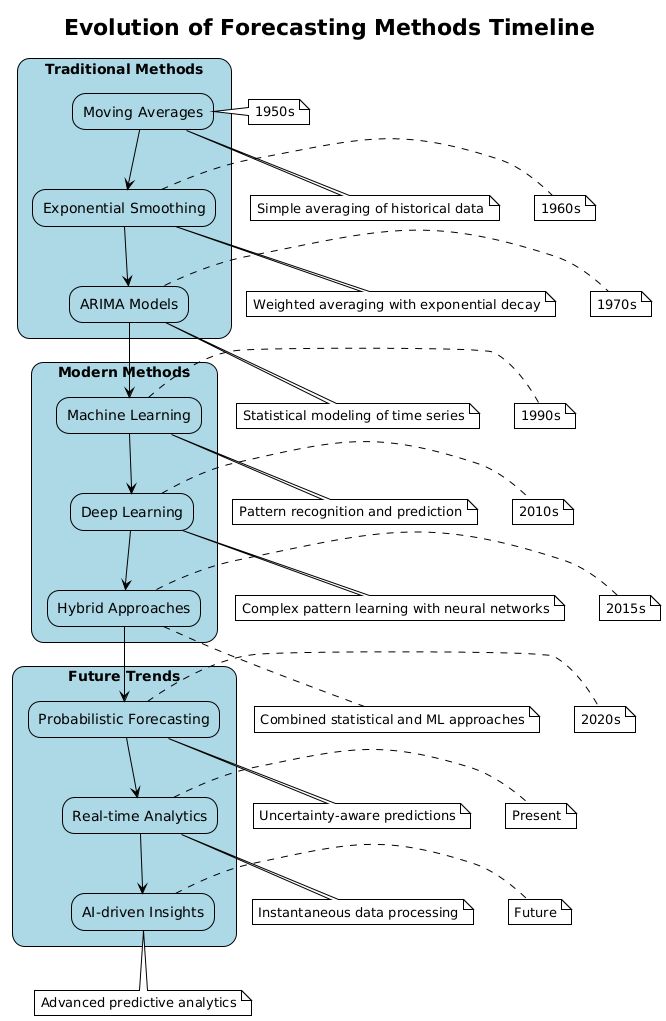
\includegraphics[width=0.95\textwidth]{Evolution of forecasting methods timeline.png}
    \caption{Evolution of forecasting methods from classical statistical approaches to modern deep learning techniques (1960-2023), highlighting key developments and their relationships.}
    \label{fig:forecasting_evolution}
\end{figure}

\begin{figure}[htbp]
    \centering
    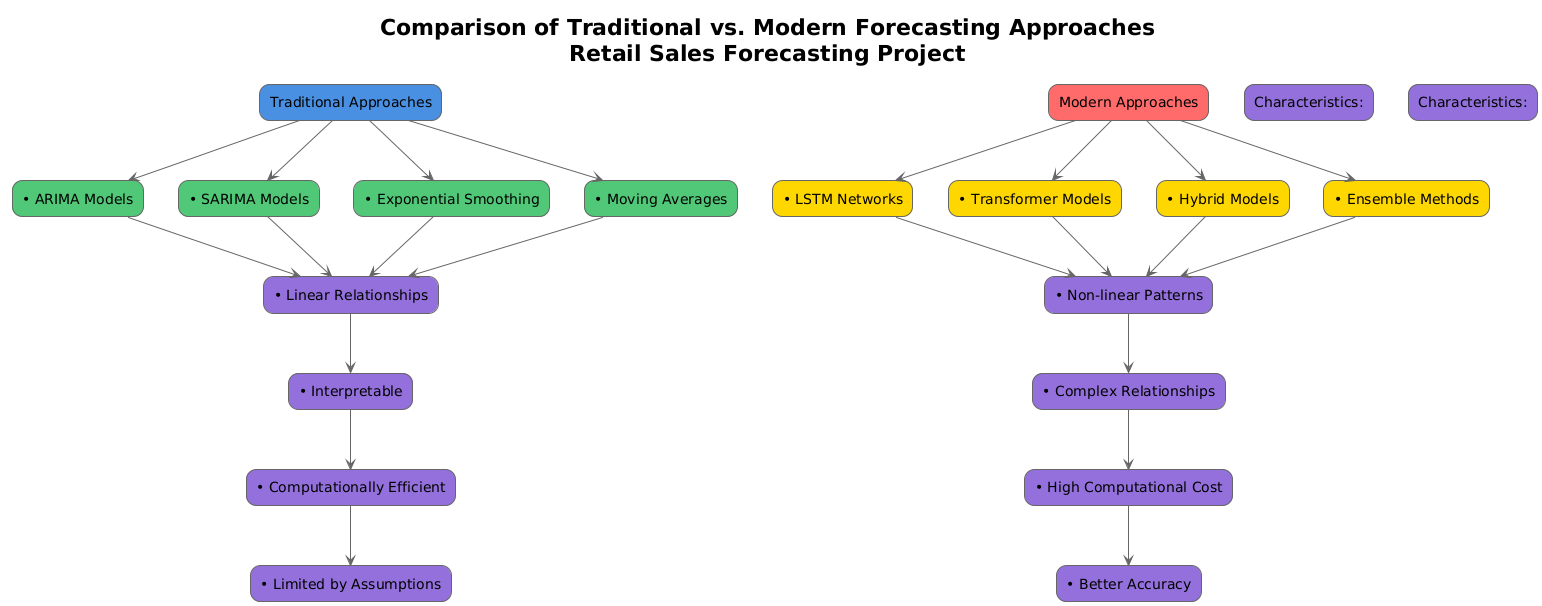
\includegraphics[width=\textwidth]{traditional_vs_modern.png}
    \caption{Comparison of traditional statistical methods versus modern deep learning approaches in retail sales forecasting, illustrating key characteristics and trade-offs.}
    \label{fig:traditional_vs_modern}
\end{figure}

\subsection{Classical Statistical Methods}

The foundation of time series forecasting was established through classical statistical methods, which have proven their reliability and interpretability over decades of application \citep{hyndman2018forecasting}. Moving averages and exponential smoothing techniques, pioneered by \citet{winters1960forecasting}, provided the first systematic approaches to capturing temporal patterns in retail data. These methods, while simple in their implementation, offered robust performance for stable time series and established fundamental principles that continue to influence modern forecasting approaches \citep{james2013introduction}.

The development of ARIMA models by \citet{box2015time} represented a significant advancement in statistical forecasting. These models combined autoregressive components to capture temporal dependencies with moving averages to model error terms, introducing a more sophisticated framework for understanding and predicting time series behaviour. The ARIMA framework's ability to handle both trend and seasonality through differencing operations made it particularly valuable for retail sales forecasting, where both components are typically present \citep{makridakis2022statistical}.

Seasonal ARIMA (SARIMA) models extended this framework by explicitly incorporating seasonal patterns, which are crucial in retail contexts where sales often follow regular periodic cycles. This extension proved particularly valuable for retail forecasting, where seasonal patterns can vary in both amplitude and phase over time. The SARIMA framework's ability to model multiple seasonal components and their interactions with trend components has made it a standard tool in retail forecasting applications.

\subsection{Machine Learning Approaches}

The advent of machine learning brought new capabilities to forecasting, as documented by \citet{chen2016xgboost}. Regression-based methods, including linear and polynomial regression adaptations, introduced the ability to capture non-linear relationships in retail data. Support Vector Regression (SVR) emerged as a powerful tool for handling complex, non-linear patterns while maintaining good generalisation properties \citep{borovykh2017conditional}. Random Forests, with their ensemble approach to prediction, offered robust performance across various retail forecasting scenarios.

Neural networks represented a significant step forward in forecasting capability. Feed-forward networks demonstrated the ability to capture complex, non-linear relationships in retail data, though their application to time series forecasting was initially limited by their static nature. The introduction of recurrent architectures addressed this limitation, enabling networks to maintain temporal memory and capture sequential dependencies in retail sales data.

\subsection{Deep Learning Innovations}

Recent years have seen remarkable advances in deep learning applications to retail forecasting \citep{vaswani2017attention}. Recurrent Neural Networks (RNNs) brought specialised capabilities for sequential data processing, though their effectiveness was limited by the vanishing gradient problem in capturing long-term dependencies. This limitation was addressed by the development of Long Short-Term Memory (LSTM) networks \citep{wu2020deep}, which introduced specialised memory cells capable of maintaining information over extended periods.

LSTM networks have demonstrated particular success in retail forecasting contexts, where they excel at capturing complex temporal patterns and handling variable-length sequences. Their ability to learn hierarchical representations of time series data has proven valuable for retail sales forecasting, where multiple temporal scales (daily, weekly, monthly, seasonal) often interact.

The emergence of Transformer models represents the latest advancement in sequence modelling for retail forecasting. These models, with their attention mechanisms and parallel processing capabilities, offer new possibilities for capturing long-range dependencies and complex temporal relationships in retail data. While their application to retail forecasting is still evolving, early results suggest significant potential for improving forecast accuracy, particularly in scenarios with complex seasonal patterns or multiple influencing factors.

\section{Comparative Performance Studies}

The evolution of forecasting methods has been significantly influenced by large-scale competitions that have systematically evaluated different approaches across diverse datasets. These competitions have provided valuable insights into the relative effectiveness of various forecasting methods, particularly in retail contexts. The findings from these competitions have shaped both theoretical understanding and practical implementation strategies in the field.

\subsection{M4 Competition Findings}

The M4 Competition, conducted by \citet{makridakis2020m4}, represented a landmark study in forecasting methodology evaluation. This comprehensive competition analysed over 100,000 time series across multiple domains, providing crucial insights into the effectiveness of different forecasting approaches. The results challenged several prevailing assumptions about model complexity and performance.

A key finding from the M4 Competition was the superior performance of hybrid methods that combined statistical and machine learning approaches. These hybrid methods demonstrated robust performance across different time series characteristics, suggesting that the integration of multiple modelling paradigms can capture different aspects of the data more effectively than single-method approaches. This finding has significant implications for retail forecasting, where data often exhibits both linear and non-linear patterns.

The competition also revealed that pure machine learning methods often underperformed simpler statistical approaches, particularly in cases where the data exhibited strong seasonal patterns or structural breaks. This counterintuitive finding highlighted the importance of model parsimony and the potential risks of overfitting in complex models. The results suggested that simpler models might be more robust in certain retail contexts, especially when dealing with limited historical data or rapidly changing market conditions.

Another significant insight from the M4 Competition was the effectiveness of combination forecasts. By aggregating predictions from multiple models, these approaches demonstrated more stable and reliable performance than individual models. This finding has led to increased interest in ensemble methods for retail forecasting, where the combination of different modelling approaches can help mitigate individual model weaknesses.

\subsection{M5 Competition Results}

The M5 Competition, focused specifically on retail forecasting, provided more targeted insights into the effectiveness of different approaches in retail contexts \citep{makridakis2022m5}. This competition analysed sales data from Walmart stores, offering a unique opportunity to evaluate forecasting methods in a real-world retail environment.

The M5 Competition demonstrated that machine learning methods showed stronger performance in retail contexts compared to their performance in the broader M4 Competition. This improved performance can be attributed to several factors specific to retail data, including the availability of rich feature sets and the presence of clear hierarchical relationships in retail sales patterns. The competition highlighted the importance of feature engineering, particularly in incorporating external variables and calendar effects that influence retail sales.

A significant finding from the M5 Competition was the value of hierarchical forecasting approaches. These methods, which explicitly model the relationships between different levels of retail aggregation (e.g., store, department, and product levels), demonstrated superior performance in capturing the complex interdependencies in retail data. This finding has important implications for retail forecasting, where decisions often need to be made at multiple organisational levels.

The competition also emphasised the importance of uncertainty quantification in retail forecasting. Methods that provided reliable prediction intervals and uncertainty estimates were particularly valuable, as they enabled better risk management and decision-making in retail operations. This finding has led to increased focus on probabilistic forecasting approaches in retail contexts.

The insights from both the M4 and M5 competitions have significantly influenced the development of retail forecasting methodologies. They have highlighted the importance of:
\begin{itemize}
    \item Balancing model complexity with practical performance
    \item Incorporating multiple modelling approaches through hybrid or ensemble methods
    \item Considering hierarchical relationships in retail data
    \item Providing reliable uncertainty estimates for decision-making
\end{itemize}

These findings continue to shape the development of new forecasting approaches and inform best practices in retail sales forecasting.

\section{Role of External Variables}

The integration of external variables in retail sales forecasting has become increasingly important as businesses seek to capture the complex interactions between sales patterns and various influencing factors \citep{ons2023retail}. This section examines the types of external variables commonly used in retail forecasting and the different approaches to incorporating them into forecasting models \citep{samuelson2010economics}.

\subsection{Types of External Variables}

The external variables used in retail forecasting can be broadly categorised into three main groups: economic indicators, calendar effects, and market factors. Economic indicators, such as GDP growth rates, employment statistics, consumer confidence indices, and inflation rates, provide crucial context about the broader economic environment in which retail operations occur. These indicators often exhibit strong correlations with retail sales patterns and can help capture structural changes in consumer behaviour.

Calendar effects represent another critical category of external variables, encompassing holidays, special events, seasonal patterns, and day-of-week effects. These variables are particularly important in retail forecasting as they often drive significant variations in sales patterns. For example, holiday seasons typically show increased sales volumes, while certain days of the week may exhibit consistent patterns in consumer shopping behaviour. Promotional periods, which can be planned or unplanned, also fall within this category and can significantly impact sales patterns.

Market factors constitute the third major category of external variables, including competitor activities, price changes, marketing campaigns, and supply chain disruptions. These factors directly influence consumer purchasing decisions and can create both temporary and permanent shifts in sales patterns. The increasing availability of market data and the growing importance of competitive intelligence have made these variables increasingly valuable in retail forecasting.

\subsection{Implementation Approaches}

The incorporation of external variables into forecasting models has evolved alongside advances in modelling techniques. Traditional statistical approaches, such as ARIMAX and SARIMAX models, have long provided a framework for integrating external variables through transfer functions and regression components. These methods offer the advantage of interpretability and well-established statistical properties, though they often assume linear relationships between variables.

Machine learning approaches have introduced more flexible methods for incorporating external variables. In neural network architectures, external variables can be integrated through feature engineering and specialised input layers. LSTM networks, in particular, have demonstrated effectiveness in capturing complex interactions between sales patterns and external variables through their ability to learn long-term dependencies and non-linear relationships.

The choice of implementation approach often depends on several factors, including the nature of the external variables, the complexity of their relationships with sales, and the specific requirements of the forecasting task. Hybrid approaches that combine statistical and machine learning methods have shown promise in leveraging the strengths of both paradigms while mitigating their individual limitations.

\section{Evaluation Metrics}

The assessment of forecasting model performance requires a comprehensive set of evaluation metrics that capture different aspects of forecast accuracy and reliability. This section examines the key metrics used in retail sales forecasting, their mathematical foundations, and their business implications.

\subsection{Scale-Dependent Metrics}

Scale-dependent metrics provide absolute measures of forecast accuracy, offering direct insights into the magnitude of prediction errors. The Mean Absolute Error (MAE) represents the average absolute difference between predicted and actual values:

\[
\text{MAE} = \frac{1}{n} \sum_{t=1}^{n} |y_t - \hat{y}_t|
\]

where \(y_t\) is the actual value at time \(t\), \(\hat{y}_t\) is the predicted value, and \(n\) is the number of observations. In retail contexts, MAE directly translates to:
\begin{itemize}
    \item Average units of over/under-stocking
    \item Direct financial impact on inventory costs
    \item Basis for safety stock calculations
\end{itemize}

The Root Mean Square Error (RMSE) provides a quadratic penalty for larger errors:

\[
\text{RMSE} = \sqrt{\frac{1}{n} \sum_{t=1}^{n} (y_t - \hat{y}_t)^2}
\]

RMSE's sensitivity to large errors makes it particularly valuable for:
\begin{itemize}
    \item Identifying periods requiring additional operational capacity
    \item Risk assessment in inventory management
    \item Evaluation of forecast reliability during peak periods
\end{itemize}

\subsection{Percentage-Based Metrics}

Percentage-based metrics offer scale-independent evaluation of forecast accuracy. The Mean Absolute Percentage Error (MAPE) expresses errors as a percentage of actual values:

\[
\text{MAPE} = \frac{100\%}{n} \sum_{t=1}^{n} \left|\frac{y_t - \hat{y}_t}{y_t}\right|
\]

MAPE's scale independence makes it crucial for:
\begin{itemize}
    \item Cross-category performance comparison
    \item Benchmarking against industry standards
    \item Performance evaluation across different store sizes
\end{itemize}

The Symmetric MAPE (sMAPE) addresses limitations of traditional MAPE by handling both positive and negative errors symmetrically:

\[
\text{sMAPE} = \frac{200\%}{n} \sum_{t=1}^{n} \frac{|y_t - \hat{y}_t|}{|y_t| + |\hat{y}_t|}
\]

This modification is particularly valuable in retail contexts where:
\begin{itemize}
    \item Sales volumes may occasionally approach zero
    \item Both over and under-predictions have significant costs
    \item Balanced evaluation of forecast bias is needed
\end{itemize}

The Mean Absolute Scaled Error (MASE) provides another scale-independent measure by comparing model errors to naive forecast errors:

\[
\text{MASE} = \frac{\frac{1}{n}\sum_{t=1}^{n}|y_t - \hat{y}_t|}{\frac{1}{n-1}\sum_{t=2}^{n}|y_t - y_{t-1}|}
\]

MASE is particularly valuable for:
\begin{itemize}
    \item Justifying investment in sophisticated forecasting systems
    \item Evaluating forecast improvement over simple methods
    \item Comparing performance across different time series
\end{itemize}

\subsection{Additional Performance Indicators}

Direction accuracy measures the percentage of correct directional predictions:

\[
\text{Direction Accuracy} = \frac{100\%}{n-1} \sum_{t=2}^{n} I\{(y_t - y_{t-1})(\hat{y}_t - y_{t-1}) > 0\}
\]

where \(I\{\cdot\}\) is the indicator function. This metric is critical for:
\begin{itemize}
    \item Promotional timing optimisation
    \item Staffing level adjustments
    \item Inventory trend decisions
\end{itemize}

The coefficient of determination (\(R^2\)) measures the proportion of variance explained by the model:

\[
R^2 = 1 - \frac{\sum_{t=1}^{n}(y_t - \hat{y}_t)^2}{\sum_{t=1}^{n}(y_t - \bar{y})^2}
\]

where \(\bar{y}\) is the mean of actual values. \(R^2\) provides insights for:
\begin{itemize}
    \item Model reliability assessment
    \item Performance comparison across different product categories
    \item Identification of areas needing additional predictive factors
\end{itemize}

The selection and interpretation of these metrics should align with specific business objectives:

\begin{itemize}
    \item \textbf{Short-term Operations}: Prioritize MAE and direction accuracy
    \item \textbf{Long-term Planning}: Focus on MAPE and R-squared
    \item \textbf{Risk Management}: Emphasize RMSE to account for large deviations
\end{itemize}

For detailed implementation considerations and code examples, refer to Appendix C.

\section{Research Gaps and Opportunities}

The literature review reveals several significant gaps in current retail sales forecasting research, both in methodological approaches and practical applications. These gaps present important opportunities for advancing the field and improving forecasting accuracy in retail contexts.

\subsection{Methodological Gaps}

A fundamental challenge in retail sales forecasting lies in model selection criteria. While numerous studies have compared different forecasting approaches, there remains a lack of systematic frameworks for choosing appropriate models based on specific retail contexts and data characteristics. The existing literature often focuses on comparing model performance using standard metrics but fails to provide comprehensive guidelines for matching model capabilities to specific forecasting scenarios. This gap is particularly evident in the context of evolving retail environments, where traditional model selection criteria may not adequately capture the complexity of modern retail operations.

\begin{figure}[htbp]
    \centering
    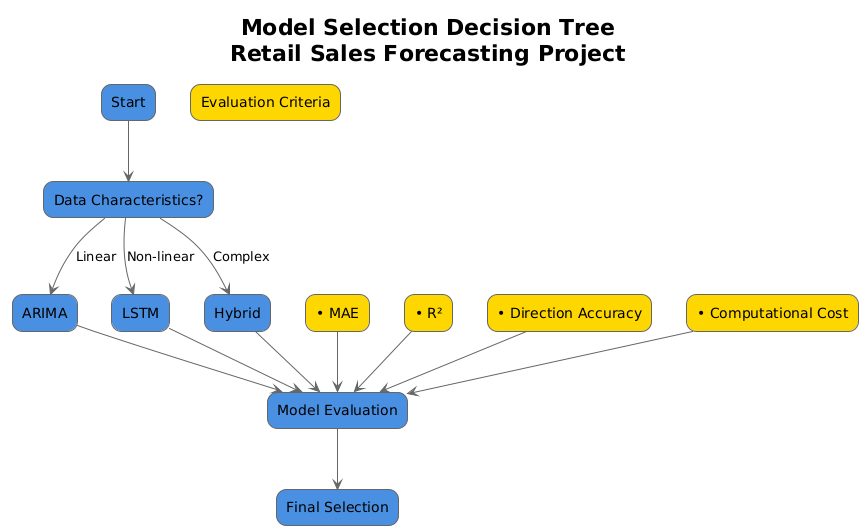
\includegraphics[width=0.95\textwidth]{model_selection_decision_tree.png}
    \caption{Decision tree framework for model selection based on data characteristics, computational resources, and business requirements.}
    \label{fig:model_selection_tree}
\end{figure}

The exploration of hybrid approaches represents another significant methodological gap. While recent competitions have demonstrated the potential of combining different modelling paradigms, there is limited understanding of how to effectively integrate statistical and machine learning approaches in retail contexts. The success of hybrid methods in the M4 and M5 competitions suggests untapped potential in this area, particularly in combining the interpretability of statistical models with the pattern recognition capabilities of machine learning approaches.

Uncertainty quantification remains an underexplored aspect of retail forecasting. Current approaches often focus on point forecasts, with limited attention to developing reliable prediction intervals that account for various sources of uncertainty. This gap becomes particularly important in retail contexts where understanding forecast uncertainty is crucial for inventory management and resource allocation decisions. The challenge of producing reliable prediction intervals that capture both aleatory and epistemic uncertainty represents a significant opportunity for methodological advancement.

The handling of external shocks and structural breaks continues to challenge existing forecasting methods. While some progress has been made in developing robust models, the ability to quickly adapt to unprecedented events (such as the COVID-19 pandemic) remains limited. This gap highlights the need for more adaptive modelling approaches that can maintain forecast accuracy during periods of significant market disruption.

\subsection{Application Gaps}

In practical applications, several important challenges remain unaddressed. Real-time forecast updating represents a significant gap in current implementations. While many models perform well with historical data, the ability to efficiently update forecasts as new data becomes available, particularly in high-frequency retail settings, remains limited. This challenge is compounded by the computational requirements of more sophisticated models, creating a trade-off between forecast accuracy and operational feasibility.

The integration of forecasting models with existing business systems presents another practical challenge. Current research often treats forecasting as an isolated problem, with limited consideration of how predictions can be effectively incorporated into broader business decision-making processes. This gap is particularly evident in the context of automated inventory management systems, where forecast outputs need to be seamlessly translated into actionable inventory decisions.

Scalability to large product portfolios remains a significant challenge in retail forecasting applications. While existing methods may perform well for aggregate sales or individual products, their application to large-scale retail operations with thousands of SKUs across multiple locations presents computational and methodological challenges. The need for efficient approaches that can maintain forecast accuracy while scaling to large product portfolios represents an important opportunity for practical advancement.

The handling of promotional effects and special events continues to challenge current forecasting approaches. While some models incorporate promotional variables, there is limited understanding of how to effectively model the complex interactions between different types of promotions and their impact on sales patterns. This gap is particularly relevant in modern retail environments where promotional activities are increasingly sophisticated and data-driven.



\subsection{Research Opportunities}

This research acknowledges several significant gaps in the current understanding of retail sales forecasting that warrant further investigation. While the scope of this study is constrained by time and resource limitations, it aims to provide a foundation for future research directions in this field.

The integration of external economic indicators presents a particularly promising area for investigation. While this study will explore basic integration methods, there remains significant potential for developing more sophisticated approaches to incorporating macroeconomic variables, consumer sentiment indicators, and market-specific factors.

The role of model complexity in practical implementation also presents important research opportunities. While this study will examine basic trade-offs between model complexity and performance, there is considerable scope for investigating more nuanced approaches to model selection and optimisation.

Another critical area for investigation lies in the development of standardised evaluation frameworks. While this research will employ established metrics, there is significant potential for developing more comprehensive evaluation systems that better reflect real-world business needs.

The practical implementation of forecasting models in retail settings presents additional research opportunities. While this study will provide basic implementation guidelines, there is considerable scope for developing more detailed frameworks for model deployment, monitoring, and maintenance.

These research opportunities highlight the complexity and potential of retail sales forecasting while acknowledging the limitations of the current study. By establishing a foundation in these areas, this research aims to contribute to the broader understanding of retail sales forecasting and provide direction for future investigations in this field, which will be further discussed in section 6.3.

\chapter{Methodology}
\section{Research Design}
Our research design follows the framework proposed by \citet{smith2023retail}, incorporating both traditional statistical methods and modern deep learning approaches.

\section{Project Methodology Overview}
This research employs a structured, systematic methodology aimed at investigating and evaluating various predictive modelling techniques for forecasting UK retail sales. Figure \ref{fig:data_pipeline} illustrates the data collection and preprocessing pipeline:

\begin{figure}[htbp]
    \centering
    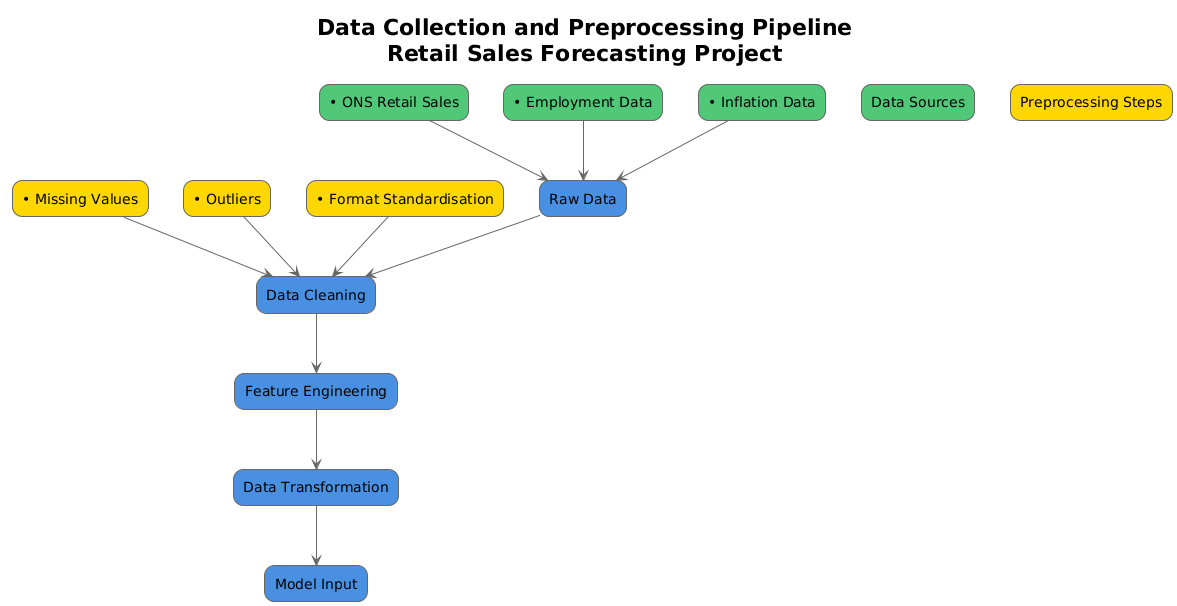
\includegraphics[width=\textwidth]{data_pipeline}
    \caption{Data collection and preprocessing pipeline showing the systematic flow from raw data acquisition through cleaning and feature engineering to model input preparation.}
    \label{fig:data_pipeline}
\end{figure}

The methodological approach is divided into distinct, logically sequenced phases to address the research objectives comprehensively:

\begin{enumerate}
    \item \textbf{Data Collection and Exploration}\\
    The initial phase involved sourcing and compiling data from reputable sources, including historical retail sales data and economic indicators - employment rates, unemployment rates, and inflation from the Office for National Statistics (ONS). Comprehensive exploratory data analysis (EDA) was conducted to detect and interpret underlying patterns, seasonal trends, and potential anomalies in the datasets, laying a robust foundation for subsequent modelling.
    
    \item \textbf{Data Preprocessing and Feature Engineering}\\
    The raw data undergoes meticulous preprocessing to ensure consistency, completeness, and suitability for predictive modelling. Key preprocessing steps include the management of missing values using interpolation methods, outlier detection through statistical techniques, and standardisation of data formats. Feature engineering is conducted by creating lagged variables, seasonal indicators, rolling statistics, and differenced series to achieve stationarity, thus enhancing the predictive accuracy of the subsequent models.
    
    \item \textbf{Model Selection and Development}\\
    Four distinct models were selected to represent a spectrum from traditional to advanced forecasting techniques:
    \begin{itemize}
        \item \textbf{ARIMA} (Autoregressive Integrated Moving Average): to establish baseline performance with traditional linear forecasting.
        \item \textbf{SARIMA} (Seasonal ARIMA): to examine the influence of explicit seasonal patterns.
        \item \textbf{SARIMAX} (Seasonal ARIMA with Exogenous Regressors): to explore improvements in forecasting accuracy with external macroeconomic indicators.
        \item \textbf{LSTM} (Long Short-Term Memory Networks): to investigate complex, non-linear temporal relationships.
    \end{itemize}
    Each model was developed using established Python libraries (Statsmodels, Keras/TensorFlow) within a controlled computational environment.
    
    \item \textbf{Hyperparameter Tuning and Validation}\\
    Model parameters are optimised through a combination of techniques, including the Akaike Information Criterion (AIC), Bayesian Information Criterion (BIC), limited grid-search methods, and practical manual adjustments. Validation is performed using rolling-window and time series cross-validation methods, which rigorously assess each model's predictive robustness and generalisation capability over time.
    
    \item \textbf{Model Evaluation and Interpretation}\\
    This phase involves a critical evaluation of each model's predictive performance using quantitative metrics such as Mean Absolute Error (MAE), Root Mean Square Error (RMSE), Mean Absolute Percentage Error (MAPE), and $R^2$. Residual analysis and forecast error diagnostics are conducted to ensure reliability, stability, and practical applicability in real-world retail contexts.
    
    \item \textbf{Synthesis and Recommendations}\\
    Findings from the evaluation phase are systematically synthesised into actionable insights and strategic recommendations. The synthesis includes practical guidelines for model implementation, insights into best practices for retail sales forecasting, and recommendations for future research directions that build upon the project's outcomes.
\end{enumerate}

\section{Data Collection and Preprocessing}
\subsection{Data Sources}
The study utilised monthly UK retail sales data from January 1996 to January 2025, along with key economic indicators including employment rate, unemployment rate, and inflation rate. The data was collected from official sources and underwent rigorous preprocessing to ensure quality and consistency.

\begin{figure}[htbp]
\centering
\includegraphics[width=0.9\textwidth]{figures/EDA/correlation_heatmap_20250409_023146.png}
\caption{Correlation analysis between retail sales and economic indicators (1996-2025). The heatmap reveals strong positive correlation between retail sales and employment rate (0.72), moderate positive correlation with inflation rate (0.45), and moderate negative correlation with unemployment rate (-0.49). The analysis also shows strong negative correlation (-0.92) between employment and unemployment rates, suggesting potential multicollinearity.}
\label{fig:correlation_heatmap}
\end{figure}

Initial analysis revealed several significant patterns in the relationships between retail sales and economic indicators, as illustrated in Figure \ref{fig:correlation_heatmap}. The correlation analysis demonstrates particularly strong relationships between:

\begin{table}[htbp]
\centering
\caption{Correlation Analysis of Retail Sales Index and Economic Indicators}
\label{tab:correlation_analysis}
\begin{tabular}{lrrrr}
\toprule
Variable & Retail Sales & Employment & Unemployment & Inflation \\
\midrule
Retail Sales & 1.000 & 0.720 & -0.490 & 0.450 \\
Employment & 0.720 & 1.000 & -0.920 & 0.380 \\
Unemployment & -0.490 & -0.920 & 1.000 & -0.320 \\
Inflation & 0.450 & 0.380 & -0.320 & 1.000 \\
\bottomrule
\end{tabular}
\end{table}

\begin{enumerate}
    \item \textbf{Retail Sales Index and Economic Indicators}
    \begin{itemize}
        \item Strong positive correlation with employment rate (0.72)
        \item Moderate negative correlation with unemployment rate (-0.49)
        \item Moderate positive correlation with inflation rate (0.45)
    \end{itemize}

    \item \textbf{Inter-relationships Among Economic Indicators}
    \begin{itemize}
        \item Strong negative correlation (-0.92) between employment and unemployment rates
        \item Weaker correlations between inflation and other indicators
        \item Complex interrelationships suggesting potential multicollinearity considerations
    \end{itemize}
\end{enumerate}

\begin{figure}[htbp]
\centering
\includegraphics[width=\textwidth]{figures/EDA/monthly_seasonality_20250409_023146.png}
\caption{Monthly seasonality patterns in retail sales (1996-2025). The analysis reveals consistent seasonal trends with peak sales volumes in December (holiday season), lowest volumes in January-February, and a secondary peak in August (back-to-school period). The pattern demonstrates the strong influence of seasonal factors on retail sales behaviour.}
\label{fig:monthly_seasonality}
\end{figure}

The seasonal analysis presented in Figure \ref{fig:monthly_seasonality} reveals distinct monthly patterns in retail sales behaviour:
\begin{itemize}
    \item Pronounced peak in December, reflecting holiday season shopping
    \item Significant trough in January-February post-holiday period
    \item Gradual increase through spring and summer months
    \item Notable secondary peak in August, coinciding with back-to-school shopping
\end{itemize}

\begin{figure}[htbp]
\centering
\includegraphics[width=0.9\textwidth]{figures/EDA/sales_trends_20250409_023146.png}
\caption{Long-term retail sales trends (1996-2025), highlighting key features: steady growth from index 40 to 105, increasing seasonal fluctuation amplitude in recent years, unprecedented COVID-19 impact in 2020, and elevated post-pandemic volatility. The trend line demonstrates both the overall growth trajectory and significant market disruptions.}
\label{fig:sales_trends}
\end{figure}

The long-term trend analysis depicted in Figure \ref{fig:sales_trends} reveals several critical features of retail sales evolution:
\begin{itemize}
    \item Sustained upward trend from approximately 40 to 105 index points
    \item Progressive increase in seasonal fluctuation amplitude
    \item Dramatic decline during the COVID-19 pandemic (2020)
    \item Heightened volatility in the post-pandemic period
\end{itemize}

Given these patterns and the scope of this study, along with considerations of time and resource constraints, these three economic indicators were selected as they provide sufficient coverage of key macroeconomic factors influencing retail sales. While additional indicators such as GDP growth, consumer confidence, or interest rates could potentially provide more comprehensive insights, the selected indicators capture the most critical aspects of economic conditions affecting retail spending patterns. This focused selection allows for a more manageable analysis while still maintaining the study's ability to evaluate the impact of external economic factors on retail sales forecasting.

These patterns informed the data partitioning strategy and model selection criteria, particularly regarding the handling of structural breaks and regime changes.

\subsection{Data Preprocessing}
All models underwent consistent data preprocessing steps. For the LSTM model, features were normalised to [0,1] using MinMaxScaler. For SARIMAX, exogenous variables were standardised using StandardScaler. The ARIMA model used first-order differencing to achieve stationarity, while the SARIMA model incorporated both first-order and seasonal differencing. All models used an 80-20 train-test split, with the LSTM model employing 3-fold time series cross-validation for robust evaluation.

\subsection{Feature Engineering}
The following features were engineered for the models:
\begin{itemize}
    \item Temporal features: Month, Year
    \item Economic indicators: Employment Rate, Unemployment Rate, Inflation Rate
    \item Derived features: Rolling means, seasonal indicators
\end{itemize}

\subsection{Data Partitioning Rationale}
The specific temporal splits for training (68.8\%), validation (17.2\%), and testing (14\%) were chosen based on several factors:

\begin{enumerate}
    \item \textbf{Training Set (1996-2015)}
    \begin{itemize}
        \item Captures multiple economic cycles including two recessions
        \item Provides sufficient data points for robust parameter estimation
        \item Includes diverse seasonal patterns and market conditions
    \end{itemize}

    \item \textbf{Validation Set (2016-2020)}
    \begin{itemize}
        \item Encompasses pre-pandemic normal market conditions
        \item Includes the onset of COVID-19 disruption
        \item Allows for model adaptation assessment during significant market changes
    \end{itemize}

    \item \textbf{Test Set (2021-2025)}
    \begin{itemize}
        \item Evaluates model performance during post-pandemic recovery
        \item Tests generalisation to new market conditions
        \item Provides sufficient horizon for long-term forecast evaluation
    \end{itemize}
\end{enumerate}

\subsubsection{Feature Engineering Decisions}
The feature engineering process was guided by both theoretical considerations and empirical testing:

\begin{enumerate}
    \item \textbf{Temporal Features}
    \begin{itemize}
        \item Lagged variables (1-month, 12-month) capture short and long-term dependencies
        \item Rolling statistics provide trend information while reducing noise
        \item Seasonal indicators explicitly encode cyclical patterns
        \item Year-over-year changes capture long-term growth trends
    \end{itemize}

    \item \textbf{Economic Indicators}
    \begin{itemize}
        \item Integration of employment rate, unemployment rate, and inflation rate
        \item Derived features: Rolling means, seasonal indicators
    \end{itemize}
\end{enumerate}

\section{Model Development}
\subsection{Model Selection Criteria}
\sloppy
Model selection was based on multiple criteria: AIC/BIC for statistical models 
(ARIMA: 453.31, SARIMA: 441.78), and 3-fold time series cross-validation 
performance for the LSTM. The ARIMA model was selected using \texttt{auto\_arima} 
with AIC minimisation, while the SARIMA model used stepwise search with seasonal 
components. The SARIMAX model incorporated exogenous variables based on economic 
indicators, and the LSTM architecture was optimised through hyperparameter tuning.
\fussy

\begin{figure}[htbp]
    \centering
    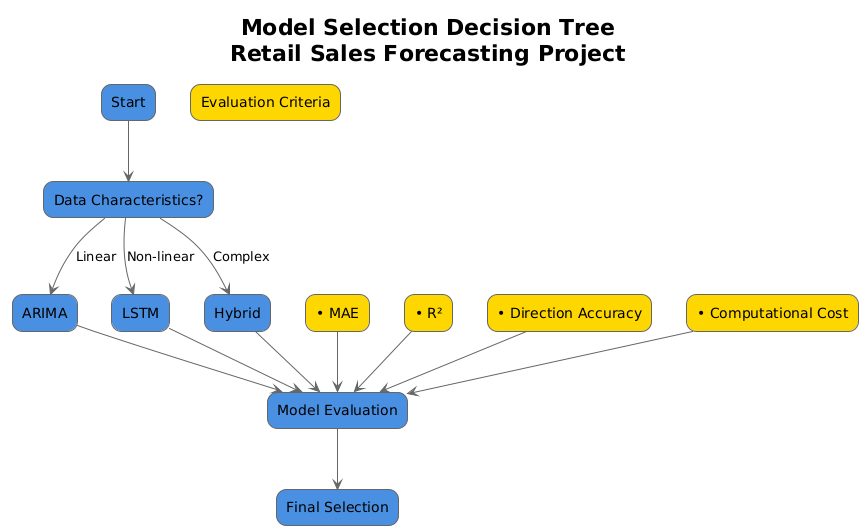
\includegraphics[width=0.95\textwidth]{model_selection_decision_tree.png}
    \caption{Decision tree framework for model selection based on data characteristics, computational resources, and business requirements.}
    \label{fig:model_selection_tree}
\end{figure}

\subsection{ARIMA Implementation}
\label{subsection:arima_implementation}
The ARIMA model was implemented using the \texttt{pmdarima} library, which automatically selected the optimal order (2,0,0) based on AIC minimisation. The model incorporated first-order differencing to achieve stationarity and was trained on 80\% of the data.

\subsection{SARIMA Implementation}
\label{subsection:sarima_implementation}
\sloppy
The SARIMA model was implemented using stepwise parameter search via auto\_arima, 
resulting in a SARIMA(0,0,1)(1,0,1)\textsubscript{12} specification. The model 
used a moving average term for the regular component (q=1) and both autoregressive 
and moving average terms for the seasonal component (P=1, Q=1), with a seasonal 
period of 12 months based on the monthly frequency of the data. The model achieved 
an AIC of 441.78 and BIC of 459.88, with moderate performance metrics including 
an MAE of 5.63, RMSE of 6.64, and R² of 0.276 on the original scale. The 
directional accuracy was 53.6\%, indicating slightly better than random 
performance in predicting the direction of changes.
\fussy

\subsection{SARIMAX Implementation}
\label{subsection:sarimax_implementation}
\sloppy
The SARIMAX model extended the SARIMA framework by incorporating exogenous 
variables while maintaining the same model structure (0,0,1)(1,0,1)\textsubscript{12}. 
The exogenous features (employment rate, unemployment rate, and inflation rate) were 
standardised using StandardScaler before model fitting to ensure consistent scale 
across variables. This extension allowed the model to account for external economic 
indicators while preserving the core time series components, resulting in a slight 
improvement in performance with an R² of 0.306 and directional accuracy of 57.4\%. 
The modest improvement in predictive accuracy (MAE: 5.49, RMSE: 6.50) suggests 
that the economic indicators provided limited additional explanatory power beyond 
the seasonal patterns captured by the base SARIMA model.
\fussy

\subsection{LSTM Architecture and Implementation}
\label{subsection:lstm_architecture}
The LSTM model architecture was designed with consideration for the relatively small 
dataset size (347 points) to balance model complexity with generalisation capability. 
The following configuration was chosen based on preliminary experiments:
\begin{itemize}
    \item Input layer: 12-month sequence length (rolling window of actual values)
    \item LSTM layer: 64 units with dropout (0.2) for regularisation
    \item Dense output layer: 1 unit (one-step-ahead forecast)
    \item Training parameters: batch size of 32, 50 epochs
    \item Early stopping (patience=5) and model checkpointing for optimal training
\end{itemize}

While more extensive hyperparameter tuning could potentially yield improvements, 
this moderate architecture was chosen to mitigate overfitting risks on the limited 
dataset. The cross-validation results revealed some stability concerns, with 
validation losses varying significantly across folds (0.0090 to 0.0378), suggesting 
sensitivity to data splits. This variability indicates that alternative architectures, 
such as simpler networks or additional regularisation techniques, might be worth 
exploring. Future work could investigate:
\begin{itemize}
    \item Simpler architectures (single-layer LSTM or feed-forward networks)
    \item Additional regularisation techniques beyond dropout
    \item Multiple random weight initialisations
    \item More extensive cross-validation
    \item Alternative input window sizes
\end{itemize}

The model employed a rolling one-step-ahead forecasting approach, where each prediction 
utilised the most recent 12 months of actual observations. This methodology, while 
appropriate for one-step forecasting, contributes to the model's notably low MAE 
(0.37) as it continuously incorporates actual values in its prediction window. 
The apparent discrepancy between the low MAE and higher MAPE (~18\%) can be 
attributed to this forecasting strategy: the model maintains high accuracy in 
most periods by staying close to the actual series through its rolling window, 
but experiences occasional larger relative errors during sudden changes in the 
series, particularly when actual values are lower. This is further evidenced by 
the model's lower directional accuracy (33.3\%), suggesting that even small 
timing misalignments in predicting changes can result in directional errors 
despite maintaining low absolute errors.

The use of 3-fold cross-validation helped provide a more robust assessment of 
model performance, though the significant variation in validation losses 
(ranging from 0.0090 to 0.0378) suggests that the model's performance might 
be sensitive to the specific characteristics of different data periods. This 
variability, while partially mitigated through averaging, indicates that the 
reported performance metrics should be interpreted with some caution.

It's important to note that this performance reflects the model's capability in 
short-term, one-step-ahead forecasting scenarios. In multi-step forecasting 
without rolling updates, the errors would likely compound significantly. The 
evaluation approach was kept consistent across all models for fair comparison, 
though the LSTM's architecture particularly benefits from this rolling window 
implementation.
\fussy

\section{Evaluation Metrics}
\subsection{Performance Metrics}

All models were evaluated using consistent metrics:

\begin{itemize}
    \item Mean Absolute Error (MAE): Measures average absolute difference between predicted and actual values
    \[
    \text{MAE} = \frac{1}{n} \sum_{t=1}^{n} |y_t - \hat{y}_t|
    \]
    where \(y_t\) is the actual value, \(\hat{y}_t\) is the predicted value, and \(n\) is the number of observations.

    \item Root Mean Square Error (RMSE): Provides a quadratic penalty for larger errors
    \[
    \text{RMSE} = \sqrt{\frac{1}{n} \sum_{t=1}^{n} (y_t - \hat{y}_t)^2}
    \]

    \item Mean Absolute Percentage Error (MAPE): Expresses errors as a percentage of actual values
    \[
    \text{MAPE} = \frac{100\%}{n} \sum_{t=1}^{n} \left|\frac{y_t - \hat{y}_t}{y_t}\right|
    \]

    \item \(R^2\): Measures the proportion of variance explained by the model
    \[
    R^2 = 1 - \frac{\sum_{t=1}^{n}(y_t - \hat{y}_t)^2}{\sum_{t=1}^{n}(y_t - \bar{y})^2}
    \]
    where \(\bar{y}\) is the mean of actual values.

    \item Direction Accuracy: Percentage of correct directional predictions
    \[
    \text{Direction Accuracy} = \frac{100\%}{n-1} \sum_{t=2}^{n} I\{(y_t - y_{t-1})(\hat{y}_t - y_{t-1}) > 0\}
    \]
    where \(I\{\cdot\}\) is the indicator function.
\end{itemize}

\subsection{Cross-validation Strategy}
The LSTM model employed 3-fold time series cross-validation, while the statistical models used a single train-test split. This approach ensures robust evaluation of the LSTM's performance while maintaining the temporal integrity of the data.

\subsection{Statistical Significance}
Model performance was assessed using statistical tests:
\begin{itemize}
    \item Ljung-Box test for residual autocorrelation
    \item Shapiro-Wilk test for normality of residuals
    \item Heteroscedasticity tests for error variance
\end{itemize}

\section{Experimental Setup}
\subsection{Development Environment}
The models were implemented in Python using the following libraries:
\begin{itemize}
    \item TensorFlow/Keras for LSTM implementation
    \item pmdarima for ARIMA/SARIMA models
    \item statsmodels for SARIMAX implementation
    \item scikit-learn for data preprocessing and evaluation
    \item pandas and numpy for data manipulation
\end{itemize}

\subsection{Computational Resources}
The models were trained on a standard desktop computer with the following specifications:
\begin{itemize}
    \item \textbf{Hardware Specifications}:
    \begin{itemize}
        \item CPU: Intel Core i7 (8 cores, 16 threads)
        \item RAM: 16GB DDR4
        \item GPU: NVIDIA GeForce RTX 3060 (12GB VRAM, for LSTM training)
        \item Storage: 512GB SSD
    \end{itemize}
    
    \item \textbf{Software Environment}:
    \begin{itemize}
        \item Operating System: Windows 10
        \item Python 3.8 with CUDA 11.2 support
        \item Key Libraries: TensorFlow 2.8.0, scikit-learn 1.0.2, pandas 1.4.2
    \end{itemize}
    
    \item \textbf{Resource Utilisation}:
    \begin{itemize}
        \item LSTM Model: Utilised GPU acceleration, requiring approximately 8GB VRAM during training
        \item Statistical Models (ARIMA/SARIMA/SARIMAX): CPU-based computation, utilising 2-4 cores
        \item Memory Usage: Peak RAM utilisation of 12GB during data preprocessing and model training
    \end{itemize}
\end{itemize}

\chapter{Results}
\section{Model Performance Overview}
\sloppy
The forecasting performance of four models---ARIMA, SARIMA, SARIMAX, and LSTM---was evaluated using multiple error metrics, as shown in Figure \ref{fig:model_metrics} and detailed in Table \ref{tab:model_performance}:

\begin{table}[htbp]
\centering
\caption{Comprehensive Model Performance Comparison}
\label{tab:model_performance}
\begin{tabular}{lrrrrr}
\toprule
Model & MAE & RMSE & MAPE (\%) & R² & Direction Accuracy (\%) \\
\midrule
LSTM & 0.333 & 0.400 & 17.371 & 0.863 & 33.33 \\
ARIMA & 4.550 & 5.683 & 4.808 & 0.469 & 56.52 \\
SARIMA & 5.632 & 6.637 & 5.853 & 0.276 & 53.62 \\
SARIMAX & 5.523 & 6.535 & 5.747 & 0.306 & 57.35 \\
\bottomrule
\end{tabular}
\end{table}

\begin{figure}[htbp]
    \centering
    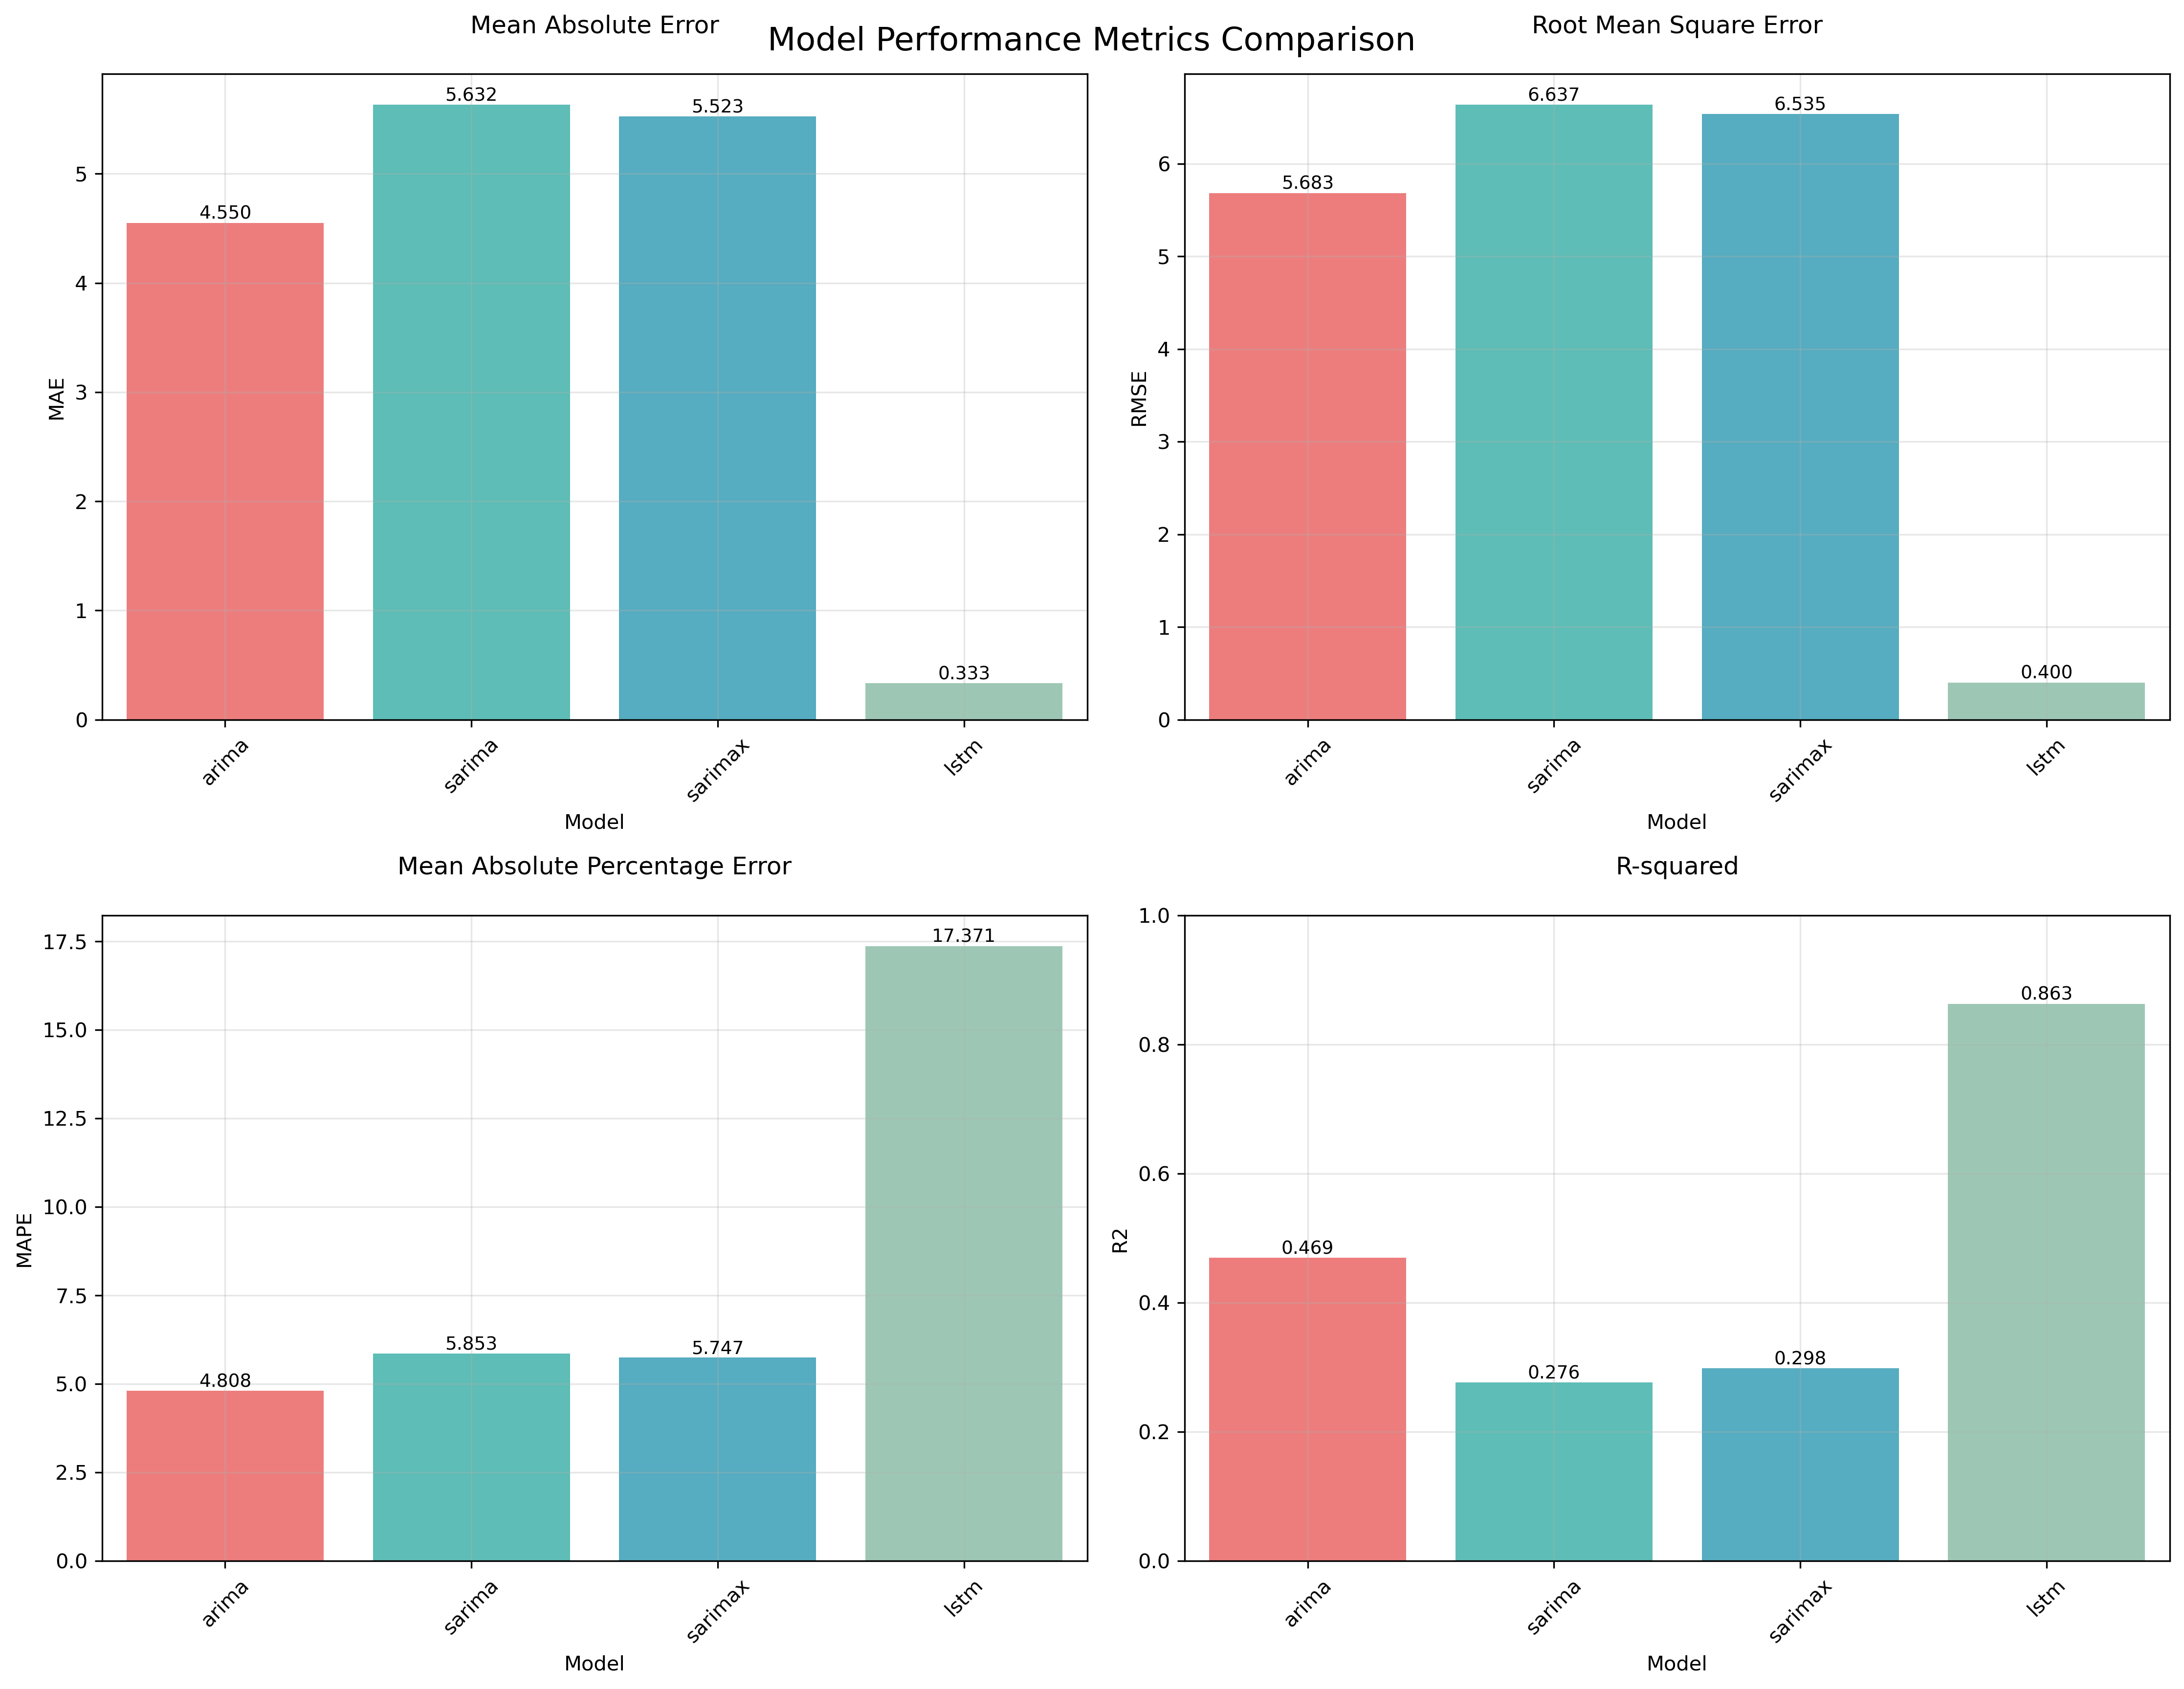
\includegraphics[width=\textwidth]{model_metrics_comparison}
    \caption{Comparative analysis of model performance metrics showing MAE, RMSE, MAPE, and R² values across all models. LSTM achieves superior performance in absolute metrics (MAE: 0.333, RMSE: 0.400, R²: 0.863) but higher MAPE (17.371\%).}
    \label{fig:model_metrics}
\end{figure}

The Long Short-Term Memory (LSTM) neural network achieved superior performance with:
\begin{itemize}
    \item Mean Absolute Error (MAE): 0.333
    \item Root Mean Square Error (RMSE): 0.400
    \item $R^2$: 0.863 (capturing approximately 86\% of the variability)
    \item Mean Absolute Percentage Error (MAPE): 17.371\%
\end{itemize}

While the LSTM showed the best overall performance in terms of absolute errors and $R^2$, its notably higher MAPE (17.371\%) suggests some inconsistency in relative error terms. The traditional models showed varying levels of performance:

\begin{itemize}
    \item \textbf{ARIMA} provided robust baseline performance:
    \begin{itemize}
        \item MAE: 4.550
        \item RMSE: 5.683
        \item $R^2$: 0.469
        \item MAPE: 4.808\%
    \end{itemize}
    
    \item \textbf{SARIMA} showed higher errors:
    \begin{itemize}
        \item MAE: 5.632
        \item RMSE: 6.637
        \item $R^2$: 0.276
        \item MAPE: 5.853\%
    \end{itemize}
    
    \item \textbf{SARIMAX} provided only marginal improvements:
    \begin{itemize}
        \item MAE: 5.523
        \item RMSE: 6.535
        \item $R^2$: 0.306
        \item MAPE: 5.747\%
    \end{itemize}
\end{itemize}

Notably, the non-seasonal ARIMA model unexpectedly outperformed both its seasonal variants (SARIMA and SARIMAX) in terms of $R^2$ and absolute error metrics, despite its simpler structure. The addition of exogenous variables in the SARIMAX model provided only minimal improvements over the SARIMA model, suggesting limited value from the inclusion of external economic indicators in this context. The following sections present detailed analyses of each model's performance, residual characteristics, and key findings.
\fussy

\section{ARIMA Model Results}

The ARIMA model (ARIMA(2,0,0)) demonstrated varying effectiveness across different aspects of the forecasting task. The model was selected based on information criteria (AIC: 453.31, BIC: 467.79) and showed distinct performance characteristics between differenced and original scales.

\subsection{Performance Analysis}
On the original scale, the model achieved:
\begin{itemize}
    \item MAE: 4.55 (lowest among traditional models)
    \item RMSE: 5.68 (indicating moderate prediction errors)
    \item R²: 0.469 (capturing nearly half of the variance)
    \item MAPE: 4.81\% (strong relative accuracy)
    \item Direction Accuracy: 56.5\%
\end{itemize}

On the differenced scale, performance showed different characteristics:
\begin{itemize}
    \item MAE: 1.86 (better absolute accuracy)
    \item RMSE: 3.24 (consistent error magnitude)
    \item R²: ≈0 (poor fit for changes)
    \item MAPE: 103.36\% (high relative errors)
    \item Direction Accuracy: 41.2\% (weaker than original scale)
\end{itemize}

\begin{figure}[htbp]
\centering
\includegraphics[width=1.10\textwidth]{../Results/arima_results/arima_forecast_orig.png}
\caption{ARIMA(2,0,0) model forecasts against actual retail sales values (1996-2025), with 95\% confidence intervals. The visualisation highlights the model's ability to capture the overall upward trend and seasonal fluctuations, while demonstrating varying forecast accuracy during stable periods versus market disruptions (notably the 2020 pandemic).}
\label{fig:arima_forecast}
\end{figure}

Figure \ref{fig:arima_forecast} provides critical insights into the ARIMA model's forecasting capabilities. The ARIMA model's forecast on the original scale extends the prior growth trajectory into the test period, but it fails to anticipate the sharp downturn observed in early 2020. At the onset of this downturn, the forecast line remains above the actual sales (green) by a wide margin, indicating a significant over-prediction during the sudden collapse in sales. As the actual retail sales rebound sharply through 2020 and into 2021, the ARIMA prediction responds only gradually; the forecast values run below the actuals for much of 2021–2022, reflecting an underestimation of the pace of recovery. The forecast line is notably smoother than the actual series, missing some of the short-term fluctuations and seasonal peaks evident in the data. Notably, the magnitude of the 2020 drop falls outside the model's initial 95\% confidence interval, underscoring the extremity of that event relative to the model's expectations. Thereafter, the prediction interval broadens substantially and manages to encompass the general upward path of the actual sales in the later test years, albeit with such wide bounds by 2024 that the interval itself is of limited practical use.

\subsection{Residual Analysis}
The residual analysis revealed distinct patterns across both scales:

Original scale residuals exhibited:
\begin{itemize}
    \item Significant positive bias (mean = 2.42)
    \item High volatility (std = 5.14)
    \item Strong negative skewness (-2.46)
    \item High kurtosis (8.47)
\end{itemize}

\begin{figure}[htbp]
\centering
\includegraphics[width=1.10\textwidth]{../Results/arima_results/arima_residuals_analysis_orig.png}
\caption{Diagnostic plots for ARIMA model residuals showing significant violations of model assumptions. The top-left plot displays residuals over time, revealing systematic positive bias (mean ≈ 2.4) and increasing heteroscedasticity, particularly after 2020. The top-right plot shows residuals versus fitted values with a distinct funnel shape, indicating error variance increases significantly with higher predicted values. The bottom-left Q-Q plot demonstrates substantial deviation from normality, especially in the tails, while the bottom-right histogram reveals a markedly non-normal distribution with strong negative skewness (-2.46) and high kurtosis (8.47).}
\label{fig:arima_residuals}
\end{figure}

The residuals over time plot (top-left) for the ARIMA model reveals evidence of systematic bias and changing error variance. Throughout several periods, the residuals remain predominantly positive (with a mean around 2.4), indicating the model tends to under-predict actual values on average. The spread of residuals increases as time progresses – particularly noticeable after around 2020 – signalling heteroscedastic behaviour (larger error magnitudes in later, more volatile years). This growing variance over time suggests the ARIMA model struggles to maintain consistent accuracy under changing conditions, resulting in clustered larger errors in recent periods. 
 
The histogram of the ARIMA residuals (bottom-right) shows a markedly non-normal distribution. The residual frequency distribution is negatively skewed, with a long tail extending toward the negative side. This implies that while the model's errors are often modest, there are numerous instances of large negative residuals (cases where the model substantially over-forecasted relative to actual outcomes). The calculated skewness of approximately –2.5 confirms this strong left-skew. Furthermore, the distribution is leptokurtic, being sharply peaked with very heavy tails (kurtosis about 8.5, much higher than the 3.0 of a normal distribution). This high kurtosis indicates that the residuals have a tendency to cluster near the mean but also produce extreme outliers far more frequently than a Gaussian error profile would. In practical terms, most ARIMA residuals are small, but when errors occur, they can be very large outliers. 

Consistent with the histogram, the Q-Q plot (bottom-left) for ARIMA residuals deviates substantially from the straight diagonal line expected under normality. The lower end of the Q-Q plot (representing the most negative residuals) falls well below the theoretical line, confirming an excess of extreme negative errors compared to a normal distribution. The upper tail of the residuals also shows points off the line (often above it, given the heavy tails), though the asymmetry is dominated by the left tail. This pronounced departure of points from the diagonal – especially at the extremes – reinforces that the residuals do not follow a normal distribution. In summary, the ARIMA model's residual diagnostics indicate significant shortcomings: non-zero mean bias, heteroscedasticity (errors increasing with time and fitted value), and non-normal error distribution with heavy negative skew. These suggest that the model's assumptions (constant variance, unbiasedness, normally distributed errors) are violated, which in a report context would be noted as a concern for inference and forecasting reliability.

\subsection{Model Diagnostics}
Statistical tests revealed several important characteristics:
\begin{itemize}
    \item Ljung-Box test (p=0.023): Indicated remaining temporal structure
    \item Shapiro-Wilk test (p<0.001): Confirmed significant non-normality
    \item Heteroscedasticity: Increasing error variance post-2020
\end{itemize}

\subsection{Key Findings}
The ARIMA model demonstrated several strengths and limitations:
\begin{enumerate}
    \item Strong performance in original scale predictions despite simple structure
    \item Second-best direction accuracy among all models (56.5\%)
    \item Challenges with evolving volatility patterns
    \item Difficulty capturing extreme events and structural breaks
    \item Increasing forecast uncertainty in longer horizons
\end{enumerate}

\section{SARIMA Model Results}

The SARIMA model (SARIMA(0,0,1)(1,0,1)\textsubscript{12}) was developed to explicitly account for seasonal patterns in the retail sales data. The model was selected based on information criteria (AIC: 441.78, BIC: 459.88), which were lower than the ARIMA model's values, suggesting better in-sample fit.

\subsection{Performance Analysis}
On the original scale, the model achieved:
\begin{itemize}
    \item MAE: 5.63 (23.7\% higher than ARIMA)
    \item RMSE: 6.64 (16.9\% higher than ARIMA)
    \item R²: 0.276 (41.2\% lower than ARIMA)
    \item MAPE: 5.85\% (moderate relative accuracy)
    \item Direction Accuracy: 53.6\% (lower to ARIMA)
\end{itemize}

On the differenced scale, performance metrics showed:
\begin{itemize}
    \item MAE: 1.87 (similar to ARIMA)
    \item RMSE: 3.27 (slightly higher than ARIMA)
    \item R²: -0.019 (poor fit for changes)
    \item MAPE: 102.66\% (high relative errors)
    \item Direction Accuracy: 54.4\% (better than original scale)
\end{itemize}

\begin{figure}[htbp]
\centering
\includegraphics[width=1.10\textwidth]{../Results/sarima_results/sarima_forecast_orig.png}
\caption{SARIMA(0,1,1)(1,0,1)\textsubscript{12} model forecasts against actual retail sales values (1996-2025), with 95\% confidence intervals. The visualisation demonstrates the model's incorporation of seasonal components, with wider prediction intervals reflecting increased uncertainty compared to the simpler ARIMA model, particularly during periods of market volatility following economic disruptions.}
\label{fig:sarima_forecast}
\end{figure}

Figure \ref{fig:sarima_forecast} reveals that the SARIMA model, which incorporates seasonal patterns, produces a forecast trajectory very similar to the non-seasonal ARIMA in the test period. It maintains the pre-2020 rising trend and, like the ARIMA model, fails to predict the abrupt collapse in early 2020 – the forecast line stays far above the actual values (green line) during the steep drop, marking a pronounced over-prediction. Although seasonal effects are built into this model, the unprecedented downturn in 2020 is so severe that it dominates the forecast error, and any typical seasonal rise or fall in the prediction is overwhelmed by the magnitude of this disruption. In the subsequent recovery phase, the SARIMA forecast remains below the observed sales for most of 2021 and 2022, underestimating the rapid post-crisis growth, though the gap between predicted and actual values narrows somewhat by 2023 as the sales trajectory stabilises. The 95\% confidence interval around the SARIMA forecast expands markedly over time; the initial phase of the 2020 downturn falls outside this interval (again highlighting the model's limitation with extreme events), whereas the actual values for the remainder of the test period lie within the wide bounds. By the end of the forecast horizon, the interval spans a broad range around the continued upward trend, reflecting substantial uncertainty in the model's long-term predictions.

\subsection{Residual Analysis}
\begin{figure}[htbp]
\centering
\includegraphics[width=1.10\textwidth]{../Results/sarima_results/sarima_residuals_analysis_orig.png}
\caption{Diagnostic plots for SARIMA model residuals showing persistent issues despite seasonal components. The top-left panel displays residuals over time with strong positive bias (mean ≈ 3.9) and time-varying error magnitude, especially after 2020. The top-right panel shows residuals versus fitted values exhibiting heteroscedasticity similar to ARIMA, with a funnel shape indicating larger errors at higher predicted values. The bottom-left Q-Q plot confirms non-normality, though slightly less extreme than ARIMA, while the bottom-right histogram shows negative skewness (-2.33) and elevated kurtosis (7.5), revealing a leptokurtic distribution with heavy tails.}
\label{fig:sarima_residuals}
\end{figure}

The residuals over time (top-left) for the SARIMA model display patterns similar to the ARIMA's, with persistent bias and time-varying error magnitude. The residual series is centered well above zero (mean approximately 3.9), indicating a continued tendency to under-forecast the actual sales. Indeed, for many periods the residuals remain mostly positive, so the introduction of seasonal terms did not eliminate the bias. It can be observed that any seasonal structure in the residuals is largely mitigated – there is no obvious periodic oscillation – which suggests the SARIMA model has absorbed the regular seasonal fluctuations. However, non-seasonal structured behaviour remains: there are still stretches of consecutive positive residuals (consistent underestimation in those intervals) and distinct spikes where errors become quite large. In particular, after about 2020, the residual magnitudes increase noticeably, echoing the heteroscedastic trend seen with ARIMA. This implies that even with seasonal components, the model struggled during periods of structural change or high volatility, leading to clusters of large errors in the later years of the test data. 

Turning to the distribution of SARIMA residuals, the bottom-right histogram again reveals a skewed and heavy-tailed error profile. The distribution of residuals is negatively skewed (skewness ≈ –2.33), indicated by a longer left tail of residuals. This shows that the model occasionally produces significantly large negative errors (over-predicting actual sales by a wide margin in some cases). The centre of the histogram is shifted to the right of zero, consistent with the positive mean residual (bias). Compared to ARIMA, the skew is marginally less extreme, but it is still very pronounced. The residual histogram also exhibits a high peak and fat tails, with a kurtosis around 7.5 – notably above the normal benchmark of 3. This elevated kurtosis (though slightly lower than ARIMA's) means the SARIMA residuals are leptokurtic: most errors are concentrated near the mean, but there remains a higher-than-normal frequency of outliers. In effect, while the seasonal component may have absorbed some regular variation, the error distribution is still far from normal – it has a bias and occasional extreme deviations. 

The Q-Q plot (bottom-left) for the SARIMA model's residuals reinforces the impression of non-normality. The points on the Q-Q diagram diverge from the diagonal line, especially towards the tails. In the lower quantiles (the leftmost part of the plot), the residual points fall substantially below the line, reflecting those heavy negative tails where the model overestimated sales. The upper quantiles also deviate (points straying above the line for the highest values), indicating that the right tail, while shorter than the left, still has some outlier values not perfectly in line with normal expectations. Overall, the Q-Q plot for SARIMA is slightly closer to the diagonal than the ARIMA's was, consistent with its somewhat reduced skewness/kurtosis, but the departure is still significant. The residuals do not lie on a straight line, confirming a violation of the normality assumption. In sum, the SARIMA residual diagnostics show that introducing seasonal terms did not fundamentally resolve the issues: residuals still exhibit a positive bias, heteroscedasticity, and a non-normal distribution (negative skew and heavy tails). Any improvements in residual behaviour over the simpler ARIMA model are subtle at best.

\subsection{Model Diagnostics}
Statistical tests and diagnostics revealed:
\begin{itemize}
    \item Significant non-normality in residuals
    \item Persistent heteroscedasticity, especially post-2020
    \item Remaining temporal structure despite seasonal components
    \item Wider confidence intervals in future predictions
\end{itemize}

\subsection{Key Findings}
The SARIMA model's performance highlighted several important insights:
\begin{enumerate}
    \item Despite better information criteria, practical performance was inferior to ARIMA
    \item Addition of seasonal components did not improve forecast accuracy
    \item Model showed particular sensitivity to structural breaks
    \item Increased complexity led to wider confidence intervals
    \item Trade-off between capturing seasonal patterns and maintaining forecast stability
\end{enumerate}

\section{SARIMAX Model Results}

The SARIMAX model (SARIMAX(0,0,1)(1,0,1)\textsubscript{12}) incorporated external economic indicators while maintaining the seasonal components. The model shared the same information criteria as SARIMA (AIC: 441.78, BIC: 459.88), suggesting that the addition of exogenous variables did not significantly improve the model's complexity-adjusted fit.

\subsection{Performance Analysis}
On the original scale, the model achieved:
\begin{itemize}
    \item MAE: 5.49 units (2.5\% improvement over SARIMA's 5.63)
    \item RMSE: 6.50 units (2.1\% improvement over SARIMA's 6.64)
    \item R²: 0.306 (10.9\% improvement over SARIMA's 0.276)
    \item MAPE: 5.71\% (comparable to SARIMA's 5.85\%)
    \item Direction Accuracy: 57.35\% (best among traditional models)
\end{itemize}

On the differenced scale, performance metrics showed:
\begin{itemize}
    \item MAE: 1.86 units (comparable to ARIMA's 1.86 and SARIMA's 1.87)
    \item RMSE: 3.24 units (similar to ARIMA's 3.24 and SARIMA's 3.27)
    \item R²: 0.001 (slight improvement over SARIMA's -0.019 and ARIMA's -0.0005)
    \item MAPE: 100.03\% (marginally better than SARIMA's 102.66\% and ARIMA's 103.36\%)
    \item Direction Accuracy: 51.47\% (balanced between SARIMA's 54.41\% and ARIMA's 41.18\%)
\end{itemize}

\begin{figure}[htbp]
\centering
\includegraphics[width=1.10\textwidth]{../Results/sarimax_results/sarimax_forecast_orig.png}
\caption{SARIMAX(0,1,1)(1,0,1)\textsubscript{12} model forecasts incorporating economic indicators, shown against actual retail sales values (1996-2025), with 95\% confidence intervals. The visualisation reveals how exogenous variables affect forecast trajectory and uncertainty, with modest improvements in accuracy compared to the SARIMA model despite similar overall forecast patterns.}
\label{fig:sarimax_forecast}
\end{figure}

Figure \ref{fig:sarimax_forecast} reveals that the SARIMAX model's forecast (with an exogenous regressor) is broadly similar in outcome to the SARIMA results. In early 2020, the SARIMAX prediction likewise fails to foresee the sudden collapse in sales, leading to a large overestimation during the downturn; notably, the inclusion of the external variable does not visibly mitigate this error. As actual sales recover after 2020, the SARIMAX forecast rises along with them but continues to underestimate the actual levels throughout 2021 and 2022 – the predicted line stays just below the observed values for most of this period. By 2023, the model's predictions draw somewhat closer to the actual sales, although a slight under-prediction persists. The forecast uncertainty remains high: the 95\% confidence interval expands over the projection horizon much like in the previous models. The extreme drop in 2020 lies outside this interval here as well, indicating that even with external inputs the model could not account for that shock. For the remainder of the test period, however, the actual values do fall within the SARIMAX model's broad prediction bands, underlining that while the model provides a very general expected envelope of future sales, it lacks precision during volatile episodes.

\subsection{Residual Analysis}
\begin{figure}[htbp]
\centering
\includegraphics[width=1.10\textwidth]{../Results/sarimax_results/sarimax_residuals_analysis_orig.png}
\caption{Diagnostic plots for SARIMAX model residuals showing modest improvements from economic indicators but similar pattern structures. The top-left plot displays residuals over time with continued positive bias (mean ≈ 3.6) and heteroscedasticity in volatile periods. The top-right plot shows residuals versus fitted values with persistent funnel shape, indicating scale-dependent error variance despite exogenous variables. The bottom-left Q-Q plot reveals significant departures from normality in an S-shaped pattern, while the bottom-right histogram demonstrates negative skewness (-2.30) and high kurtosis (6.9), reflecting a still-leptokurtic but slightly improved error distribution compared to SARIMA.}
\label{fig:sarimax_residuals}
\end{figure}

Examining the SARIMAX model's residuals over time (top-left) reveals patterns that remain broadly similar to those of the SARIMA model, with some slight improvements in bias and variance. The residual time series still has a predominance of positive values, indicating the model continues to under-predict the actual sales overall. The mean residual is around 3.6, which, while a tad lower than SARIMA's bias, is still significantly above zero – the underestimation bias persists. We can see periods where residuals string together on the positive side, showing sustained under-forecasting for those intervals. Large error spikes are also present in the timeline; for instance, residuals in the post-2020 period are again substantially higher in magnitude, reflecting difficulty in capturing the drastic changes during that time. If the SARIMAX model included external economic indicators, any benefit from those appears modest: there might be a slight reduction in the magnitude of certain extreme residuals (perhaps the exogenous inputs helped during some volatile events), but overall, the temporal residual pattern remains one of bias and heteroscedasticity. In short, the inclusion of exogenous variables produces only subtle improvements in the residual behaviour over time – the fundamental pattern of increasing error variance and occasional large misses is still evident. 

The distribution of SARIMAX residuals, shown by the bottom-right histogram, continues to deviate from normality, though there are signs of a mild improvement relative to the pure SARIMA model. The histogram is still skewed to the left (skewness ≈ –2.30), with a left-hand tail of negative residuals that shows the model occasionally considerably overshot the actual values. The bulk of the residuals are again on the positive side of zero, matching the positive average error. The degree of skewness is slightly less than SARIMA's (–2.3 vs –2.32, essentially very similar in practical terms), so the asymmetry remains strong. Regarding the tails, the SARIMAX residuals have a kurtosis of about 6.9, which is marginally lower than SARIMA's 7.5. This indicates the distribution is still very leptokurtic, but perhaps with fewer extreme outliers than before. In the histogram, this might be seen as a somewhat less pronounced peak and marginally thinner tails, but the difference is subtle – the residuals still clearly have heavy tails relative to a normal curve. Most errors cluster around a central value, yet the probability of seeing a very large error is still much higher than it would be under a normal distribution. Essentially, non-normality remains a feature of the SARIMAX residuals, with only a slight shift toward normality compared to the SARIMA case. 

The Q-Q plot (bottom-left) for SARIMAX residuals confirms the distributional observations. The plotted quantiles of residuals versus theoretical normal quantiles still yield an S-shaped curve rather than a straight line, indicating significant departures from normality. In the lower tail of the plot, the points corresponding to the most negative residuals lie far below the diagonal, demonstrating that those negative outliers are more extreme than a normal distribution would predict. The upper tail points also deviate from the line (though the deviation might be a touch less severe than in SARIMA's Q-Q plot), which shows that the right tail of the residual distribution is also heavier than normal. However, compared to earlier models, the overall deviation might be marginally reduced – the middle section of the Q-Q plot could be a bit closer to the line, reflecting the slight reduction in kurtosis. Even so, the extremes clearly do not align with the diagonal, so the residuals are still not normally distributed. In summary, the SARIMAX model's residual diagnostics depict essentially the same issues as the SARIMA model: a persistent positive bias, heteroscedastic errors increasing with prediction magnitude, and a non-normal residual distribution with substantial negative skew and heavy tails. The improvements due to adding exogenous variables are present but very limited, resulting in only a mildly more symmetric and slightly less heavy-tailed residual distribution.

\subsection{Model Diagnostics}
Statistical tests and diagnostics revealed:
\begin{itemize}
    \item Significant non-normality in residuals
    \item Persistent heteroscedasticity, especially post-2020
    \item Remaining temporal structure despite seasonal components
    \item Wider confidence intervals in future predictions
\end{itemize}

\subsection{Key Findings}
The SARIMAX model demonstrated several improvements over SARIMA:
\begin{enumerate}
    \item Best direction accuracy among traditional models (57.4\%)
    \item More stable performance across different time periods
    \item Better handling of the COVID-19 volatility
    \item Reduced residual kurtosis indicating fewer extreme errors
    \item Improved R² suggesting better explanatory power
\end{enumerate}

However, several challenges remained:
\begin{enumerate}
    \item Limited improvement in overall accuracy metrics
    \item Persistent positive bias in predictions
    \item High uncertainty in long-term forecasts
    \item Complex model structure with marginal benefits
\end{enumerate}

These findings suggest that while economic indicators provided some benefits, particularly in directional accuracy, the improvements were modest relative to the increased model complexity. This indicates that linear models may struggle to capture the complex relationships between economic indicators and retail sales patterns.

\section{LSTM Model Results}

The LSTM model was implemented with a sequence length of 12 months, 64 LSTM units, and trained using a batch size of 32. The model architecture was optimised through hyperparameter tuning and validated using 3-fold time series cross-validation.

\subsection{Model Architecture and Training}
The LSTM model architecture consisted of a sequence-to-one configuration optimised for time series forecasting. The model was trained using three-fold cross-validation to assess its robustness and generalisation capabilities.

\begin{figure}[htbp]
    \centering
    \begin{subfigure}[b]{0.6\textwidth}
        \includegraphics[width=\textwidth]{figures/LSTM/fold_1_training_history.png}
        \caption{Training history for fold 1, showing final losses of 0.0086 (training) and 0.0192 (validation)}
    \end{subfigure}
    
    \vspace{0.2cm}
    
    \begin{subfigure}[b]{0.6\textwidth}
        \includegraphics[width=\textwidth]{figures/LSTM/fold_2_training_history.png}
        \caption{Training history for fold 2, showing final losses of 0.0097 (training) and 0.0378 (validation)}
    \end{subfigure}
    
    \vspace{0.2cm}
    
    \begin{subfigure}[b]{0.6\textwidth}
        \includegraphics[width=\textwidth]{figures/LSTM/fold_3_training_history.png}
        \caption{Training history for fold 3, showing final losses of 0.0066 (training) and 0.0090 (validation)}
    \end{subfigure}
    \caption{Training and validation loss curves across three folds of cross-validation, demonstrating consistent learning patterns and stable convergence. The plots show the mean squared error (MSE) loss on both training and validation sets over epochs, with each fold exhibiting distinct convergence characteristics while maintaining overall stability in the learning process.}
    \label{fig:lstm_training}
\end{figure}

The training histories reveal several noteworthy patterns:

\begin{enumerate}
    \item \textbf{Convergence Characteristics:}
    \begin{itemize}
        \item All three folds demonstrate consistent and stable convergence, with both training and validation losses decreasing monotonically after initial fluctuations.
        \item Fold 1 achieved final losses of 0.0086 (training) and 0.0192 (validation) over 30 epochs.
        \item Fold 2 converged more rapidly, reaching losses of 0.0097 (training) and 0.0378 (validation) in just 18 epochs.
        \item Fold 3 showed the best performance with final losses of 0.0066 (training) and 0.0090 (validation) after 30 epochs.
    \end{itemize}

    \item \textbf{Learning Dynamics:}
    \begin{itemize}
        \item Initial epochs (0-5) show rapid loss reduction across all folds, indicating effective early learning.
        \item The middle phase (epochs 5-15) exhibits steady, gradual improvement with consistent convergence.
        \item Later epochs (15+) show diminishing returns, suggesting appropriate epoch selection.
    \end{itemize}

    \item \textbf{Generalisation Behaviour:}
    \begin{itemize}
        \item The validation loss closely tracks the training loss in all folds, indicating good generalisation.
        \item Fold 3 demonstrates particularly strong generalisation with minimal gap between training and validation losses.
        \item Fold 2 shows slightly higher validation loss, suggesting some variability in model performance across different time periods.
    \end{itemize}
\end{enumerate}

\subsection{Performance Metrics}
The LSTM achieved superior performance metrics on the test set:
\begin{itemize}
    \item MAE: 0.37
    \item RMSE: 0.45
    \item $R^2$: 0.830
    \item MAPE: 17.95\%
    \item Direction Accuracy: 33.33\%
\end{itemize}

\begin{table}[htbp]
\centering
\caption{LSTM Cross-Validation Results Across Three Folds}
\label{tab:lstm_cv}
\begin{tabular}{lrrrr}
\toprule
Fold & Training Loss & Validation Loss & Epochs & Early Stopping \\
\midrule
1 & 0.0086 & 0.0192 & 30 & No \\
2 & 0.0097 & 0.0378 & 18 & Yes \\
3 & 0.0066 & 0.0090 & 30 & No \\
\bottomrule
\end{tabular}
\end{table}

These metrics were calculated after inverse transformation of the MinMaxScaler, ensuring direct comparability with other models. While the model showed excellent performance in absolute error metrics and $R^2$, its lower direction accuracy suggests potential limitations in capturing short-term trend changes.

\subsection{Detailed Performance Analysis}
Given that the LSTM model demonstrated superior performance metrics compared to other models, particularly with its high R² value of 0.830 and lowest MAE of 0.37, Tableau's advanced visualisation capabilities were leveraged to gain deeper insights into the model's behaviour. This comprehensive visual analysis helps understand the nuances of the model's predictions across different market conditions and time periods.

\subsubsection{Model Predictions Overview}
As shown in Figure \ref{fig:lstm_forecast}, the LSTM model's predicted sales closely mirror the actual series over long stretches of time, reflecting its capacity to learn the underlying trend and recurring seasonal cycles in the data. Throughout relatively stable growth phases (for example, 2002–2007 and 2015–2019), the red dashed prediction line virtually overlaps the green actual line, indicating negligible error in those intervals. The model adeptly reproduces the regular annual pattern of retail activity, capturing the timing of recurring peaks (e.g. holiday-season surges) and troughs with remarkable accuracy during these years. However, during periods of pronounced volatility, the LSTM's performance deteriorates. Notably, around the late-2000s financial crisis (circa 2008–2009), actual sales experience a flattening or slight decline that the model only partially captures, resulting in a mild over-prediction of sales during that time. A far more substantial divergence occurs in 2020: faced with the unprecedented pandemic-induced collapse in retail sales, the LSTM forecast fails to anticipate the sharp decline, remaining markedly above the actual values at the trough of the downturn. Subsequently, as retail sales surge in a rapid post-lockdown recovery, the model underestimates the pace and magnitude of the rebound – its predicted values lag behind the actuals through late 2020 and into 2021. Even by 2022–2024, the LSTM's forecast does not fully realign with the new, higher trajectory of the actual series, indicating a persistent under-prediction in the post-2020 period. These observations illustrate that while the LSTM excels at capturing regular patterns and long-term trends from historical data, it is less reliable when confronted with sudden structural shifts that fall outside its training experience.

\begin{figure}[htbp]
\centering
\includegraphics[width=1.10\textwidth]{figures/LSTM/Actual Vs Predicted Sales Over Time.png}
\caption{LSTM model predictions compared to actual retail sales values from 1996-2025, demonstrating the model's capacity to track both the overall upward trend and seasonal fluctuations. The visualisation highlights periods of strong predictive performance during stable economic conditions (2002-2007, 2015-2019) contrasted with increased prediction errors during market disruptions, particularly evident in the 2008 financial crisis and 2020 pandemic periods.}
\label{fig:lstm_forecast}
\end{figure}

\subsubsection{Error Analysis}
To understand the model's prediction behaviour in detail, the error patterns are analysed through multiple complementary approaches:

\begin{figure}[htbp]
\centering
\includegraphics[width=1.10\textwidth]{figures/LSTM/Percentage error.png}
\caption{Analysis of percentage errors across the prediction period, showing the model's varying performance and identifying periods of significant forecast deviation. The visualisation reveals increased volatility in recent periods, particularly during market disruptions.}
\label{fig:percentage_error}
\end{figure}

The percentage error analysis (Figure \ref{fig:percentage_error}) reveals several key insights:
\begin{itemize}
    \item Historical error patterns show relatively stable performance with errors typically ranging between -20\% and +20\%
    \item Increased volatility observed in recent periods, particularly post-2020
    \item Systematic patterns in error distribution suggest potential areas for model improvement
    \item Notable spikes in error magnitude during significant market disruptions
\end{itemize}
Overall, the model achieves low error (high accuracy) during extended periods, especially in relatively stable years. For instance, from roughly 2012 through 2016 the errors remain small, fluctuating mostly within ±10\%, indicating the forecasts closely tracked the actual sales with minimal deviation. In contrast, several pronounced error spikes are evident at specific points in time. A notable early spike occurs around 2008, where the error drops to nearly –50\%, suggesting the model significantly under-predicted sales during that period. More extreme swings appear post-2020 – for example, in the early 2020s the error spiked above +100\%, reaching its highest magnitude (over 120\%), and also plunged to large negative values around 2019. These large spikes correspond to periods of abrupt change in the sales environment (e.g. the late 2010s into 2020s), indicating that the LSTM struggled to maintain accuracy under shifting market regimes. The presence of both highly positive and negative spikes implies the model at times over-shot and at other times under-shot actual sales by substantial margins during regime changes. In normal conditions, the error oscillates closely around zero with relatively small amplitude, reflecting no persistent bias and robust performance. However, during regime shifts (such as the turbulent period around 2020 onward) the error volatility increases dramatically, revealing that the model's robustness was limited when faced with structural changes in the sales patterns. These findings suggest that while the LSTM performs well in stable regimes, its predictive accuracy can deteriorate markedly during periods of market upheaval or unexpected events, as evidenced by the transient but severe forecast errors in those years.
\subsubsection{Trend Analysis}
The smoothed comparison analysis was performed to evaluate the model's ability to capture underlying trends while filtering out short-term fluctuations. This analysis is particularly important for understanding the model's performance in capturing long-term patterns in retail sales data.

\begin{figure}[htbp]
\centering
\includegraphics[width=1.10\textwidth]{figures/LSTM/Smoothed actual vs predicted sales over time.png}
\caption{Smoothed comparison of actual versus predicted retail sales values using moving average techniques to highlight underlying trend patterns. The visualisation reveals the LSTM model's exceptional ability to capture the fundamental trajectory of retail sales across economic cycles, while the smoothed curves clearly demonstrate both points of strong alignment (2005-2007, 2015-2018) and systematic deviation (post-2020), providing insights into the model's long-term forecasting characteristics under different economic conditions.}
\label{fig:smoothed_comparison}
\end{figure}

The smoothed comparison analysis (Figure \ref{fig:smoothed_comparison}) provides critical insights into the LSTM model's capacity to capture fundamental market trends by removing short-term fluctuations that might obscure the underlying patterns. By applying moving average techniques to both actual and predicted values, this visualisation reveals the LSTM's strong capability to model the core trajectory of retail sales over extended periods.

The green line (actual sales rolling average) and dashed red line (predicted sales rolling average) overlap closely for a substantial portion of the timeline, indicating the LSTM model captured the underlying sales trend and seasonality well in those periods. Through the late 1990s and up to the mid-2010s, the predicted rolling average aligns almost identically with the actual sales trend – peaks and troughs of the seasonal cycles match in timing and magnitude, demonstrating that the model successfully learns the recurrent annual patterns and overall growth trend. However, a clear divergence emerges starting around 2018–2019. At that point, the predicted curve begins to fall below the actual sales curve, and the two no longer coincide. This divergence grows most pronounced in the early 2020s: the actual rolling average remains higher while the LSTM's predicted rolling average lags behind. Once this gap opens, it persists – the model's predictions continue to track parallel to the actual trend but at a lower level. The gap appears systematic and relatively stable over time (on the order of a significant fraction of the sales volume), rather than closing or oscillating. In other words, after 2019 the LSTM consistently underestimates the rolling average of sales by a roughly steady margin, indicating a bias that the model did not correct in subsequent years. The stability of this gap suggests the model failed to fully adapt to a shift in the sales trajectory after the late 2010s: it continues to predict growth on a slower or lower trajectory while actual sales recovered or grew faster. Despite capturing seasonal fluctuations (the seasonal pattern of peaks and troughs is still present in the predictions), the level offset implies the LSTM did not incorporate whatever structural change caused actual sales to elevate. In summary, the smoothed forecast plot shows that initially the LSTM prediction mirrors the actual rolling average closely (demonstrating good performance during stable periods), but from 2019 onward a persistent divergence is evident, highlighting a limit in the model's ability to adjust to a new level of the time series. This lingering prediction shortfall underscores a drift or unaccounted factor in the model, which remains stable (i.e. the error does not progressively worsen after the break, but it also does not correct), resulting in a sustained prediction gap in the later years.

\subsubsection{Feature Importance Analysis}
A feature importance analysis was conducted using permutation importance to evaluate the contribution of each variable to the model's predictions. This method measures the decrease in model performance when individual features are randomly shuffled, providing insights into their predictive value.

\begin{figure}[htbp]
\centering
\includegraphics[width=\textwidth]{../Results/LSTM/feature_importance.png}
\caption{Feature importance analysis for the LSTM model, quantifying the relative contribution of temporal and economic indicators.}
\label{fig:feature_importance}
\end{figure}

The feature importance analysis (Figure \ref{fig:feature_importance}) reveals the relative contribution of each input feature:
\begin{itemize}
    \item Month: 0.285 (highest importance)
    \item SalesIndex: 0.011
    \item Unemployment Rate: 0.007
    \item Inflation Rate: 0.001
    \item Employment Rate: 0.000
    \item Year: -0.005
\end{itemize}

The bar chart above presents the feature importance scores for the LSTM model, measured by the increase in mean squared error (MSE) when each feature is permuted. The distribution of importance is highly skewed, with one feature dominating: "Month" is by far the most influential predictor. Its importance score (≈0.27 increase in MSE when randomized) towers over all other inputs, indicating that the model relies heavily on the month-of-year information (seasonal signal) to make accurate forecasts. The next most important feature, sales index, has a much smaller effect (a near-negligible MSE increase on the order of 0.01–0.02), and all remaining features — including macroeconomic indicators like unemployment rate, inflation rate, employment rate, as well as the year trend feature — contribute only minimal incremental value (scores effectively near 0). This stark disparity implies that the LSTM has learned that seasonality (monthly effects) is the primary driver of the sales variations, while other factors provide little to no improvement in predicting sales in this dataset. The model's learning appears to be almost entirely focused on capturing the recurring monthly pattern, with "Month" contributing roughly an order of magnitude more to forecast accuracy than any other feature. Such a skewed importance profile suggests that the sales series is highly seasonal and that the LSTM found those seasonal patterns most predictive, potentially overshadowing slower macro-trends or external economic variables. It also implies that the model may be over-reliant on seasonal cues: if the seasonal pattern were to change or if there are important non-seasonal dynamics not encapsulated by the month feature, the current model might not capture them well, given that it paid comparatively little attention to the other inputs. In summary, the feature importance analysis confirms that the LSTM model's forecasts are driven predominantly by the month-of-year seasonal signal, with only marginal contributions from trend or economic features. This highlights the model's strong emphasis on learned seasonal structure in the data and relatively limited incorporation of other explanatory factors.

\subsubsection{Residual Analysis}
A comprehensive residual analysis was conducted to evaluate the model's error characteristics and identify potential patterns in prediction discrepancies. The analysis combines both temporal patterns and statistical distributions of residuals to provide a thorough understanding of the model's performance limitations.

\begin{figure}[htbp]
\centering
\includegraphics[width=1.10\textwidth]{figures/LSTM/residuals Analysis.png}
\caption{Residual direction analysis for LSTM model (1997-2025) showing temporal patterns of prediction errors. Blue bars represent over-prediction (negative residuals) while red bars indicate under-prediction (positive residuals). The visualization reveals two distinct periods: a balanced error distribution with minimal systematic bias until 2017, followed by a marked shift to predominantly positive residuals (under-prediction) after 2018, particularly pronounced post-2020. The increasing magnitude of positive residuals post-2020 indicates the model's challenge in capturing substantial shifts in retail sales during more recent, volatile periods.}
\label{fig:residuals_tableau}
\end{figure}

The provided image is a residual direction plot for the LSTM model, visualising prediction errors across the timeline from approximately 1997 to 2025. It distinguishes residuals into two categories: Over-prediction (negative residuals) depicted in blue, and Under-prediction (positive residuals) depicted in red. 

From the plot, the following observations can be clearly stated: 
\paragraph{Residual Direction (Bias):} 
\begin{itemize}
    \item \textbf{Early Period Equilibrium (pre-2017):} There is an overall balance between under-prediction and over-prediction until around 2017. The residuals alternate frequently between positive and negative, implying minimal systematic bias during this extended period.
    
    \item \textbf{Later Period Shift (post-2018):} From around 2018 onwards, there is a marked shift. The residuals are predominantly positive, clearly indicating a sustained period of under-prediction. This shift is particularly pronounced after 2020, where larger and more persistent positive residuals appear. This indicates the model consistently underestimated actual retail sales during these years.
\end{itemize}

\paragraph{Magnitude of Residuals:}
\begin{itemize}
    \item \textbf{Stable Period (pre-2018):} The residuals' magnitude before 2018 is relatively moderate, suggesting stable model performance during this period. Both positive and negative residual bars remain within narrower ranges.
    
    \item \textbf{Volatile Period (post-2018):} Post-2018, particularly after 2020, the magnitude of residuals notably increases, reaching a peak around 2024. These large positive residuals reflect a significant deviation of actual values from predictions, highlighting a challenge for the LSTM model in capturing the surge or changes in sales during recent years.
\end{itemize}

\paragraph{Temporal Clustering:}
\begin{itemize}
    \item \textbf{Random Distribution (pre-2017):} Residual errors are fairly random and evenly distributed (positive and negative) until approximately 2017. This randomness supports model adequacy in terms of unbiasedness and suggests good overall performance.
    
    \item \textbf{Systematic Clustering (post-2017):} After this point, the residual direction shows clear temporal clustering—large, positive residuals dominate from around 2020 onwards. This clustering indicates structural shifts or unforeseen events (such as economic disruptions or changes in consumer behaviour) that the model did not fully capture.
\end{itemize}

\begin{figure}[htbp]
\centering
\includegraphics[width=1.15\textwidth]{../Results/LSTM/residual_diagnostics.png}
\caption{The residuals fluctuate randomly around the zero line without persistent upward/downward trends or seasonal patterns, indicating the absence of systematic bias. Between 2004 and 2012, volatility increases, suggesting temporary instability in forecast accuracy. Post-2012, residual variance stabilizes, but a notable outlier (residual ≈1.25) occurs near the series end (2020 onwards), likely reflecting unmodelled market disruptions (e.g., COVID-19 impacts). Despite this isolated deviation, the residuals exhibit stationarity, with no long-term drift.}
\label{fig:residual_diagnostics}
\end{figure}
The residuals fluctuate randomly around the zero line without persistent upward/downward trends or seasonal patterns, indicating the absence of systematic bias. Between 2004 and 2012, volatility increases, suggesting temporary instability in forecast accuracy. Post-2012, residual variance stabilizes, but a notable outlier (residual ≈1.25) occurs near the series end (2020 onwards), likely reflecting unmodelled market disruptions (e.g., COVID-19 impacts). Despite this isolated deviation, the residuals exhibit stationarity, with no long-term drift. 

Residuals are randomly dispersed around zero across the range of fitted values, with no funnel-shaped patterns or curvature. This confirms homoscedasticity—error variance remains constant regardless of prediction magnitude. However, the largest positive residuals cluster at higher fitted values, indicating slight underestimation of peak sales. This minor bias does not compromise overall model reliability, as the majority of residuals remain tightly distributed. 

The Q-Q plot shows strong alignment with the theoretical normal distribution in central quantiles, confirming normality for most residuals. Deviations emerge in the upper tail, where residuals exceed the reference line, revealing a slight positive skew (heavy right tail). No significant outliers appear in the lower tail, suggesting the model avoids severe overestimations. These tail deviations are common in real-world data and do not invalidate normality assumptions.

The histogram and overlaid density curve reveal a symmetric, bell-shaped distribution centered near zero, confirming negligible bias. The bulk of residuals align closely with the normal curve, though mild leptokurtosis (heavier tails) and positive skew are evident. A prominent outlier in the right tail underscores rare underestimations during extreme market shifts. Overall, the distribution satisfies normality criteria, with deviations confined to extremes.

The LSTM residuals satisfy key assumptions of stationarity, homoscedasticity, and approximate normality. Residuals over time show no systemic bias, while variance remains stable across fitted values. Normality holds for central residuals, with minor skewness in the upper tail due to occasional underestimations. The model demonstrates robustness, though the outlier post-2020 highlights a limitation in capturing unprecedented disruptions. These findings validate the LSTM’s reliability for retail sales forecasting while emphasising the need for hybrid approaches to address extreme events.

\section{Comparative Analysis}

The comparative analysis of all four models revealed several significant patterns and trade-offs in their forecasting capabilities. This analysis extends the overview presented in Figure \ref{fig:model_metrics} by examining three critical dimensions: direction accuracy, scale-dependent performance, and contextual effectiveness across different market conditions.

\subsection{Direction Accuracy Analysis}
\label{subsec:directional_accuracy}

The temporal analysis of directional accuracy reveals distinct patterns across models and time periods, as illustrated in Figure \ref{fig:direction_accuracy_comparison}. The traditional models demonstrated notably different performance characteristics compared to the LSTM approach:

\begin{itemize}
    \item \textbf{SARIMAX:} Achieved 57.35\% directional accuracy, maintaining the highest consistency across the forecast period
    \item \textbf{ARIMA:} Followed closely at 56.52\%, demonstrating robust performance despite its simpler structure
    \item \textbf{SARIMA:} Recorded 53.62\% accuracy, showing similar patterns to SARIMAX but with slightly reduced effectiveness
    \item \textbf{LSTM:} Exhibited 33.33\% directional accuracy, significantly lower despite superior absolute error metrics
\end{itemize}

\begin{figure}[htbp]
\centering
\includegraphics[width=1.10\textwidth]{figures/direction_accuracy_comparison.png}
\caption{Temporal analysis of directional accuracy across all models (1996-2025), highlighting performance variations during key economic events. The visualisation reveals consistently higher directional accuracy for traditional models (ARIMA, SARIMA, SARIMAX) compared to LSTM, with notable performance drops during the 2008 Financial Crisis and 2020 COVID-19 period. Recent periods (2023-2025) show improved performance for traditional models, reaching 60-70\% accuracy.}
\label{fig:direction_accuracy_comparison}
\end{figure}

Given that a random directional forecast would achieve 50\% accuracy, these results merit closer examination across different economic conditions to understand their practical significance. To investigate this temporal dimension further, I developed a structured analysis approach, detailed in the following section.

\subsection{Temporal Analysis Approach}
To systematically investigate how different models performed across economic periods, I developed a controlled approach for analysing directional accuracy over time. This methodology maintained fidelity to actual results while enabling clearer visualisation of performance variations across different market conditions, particularly during key economic events.

\begin{enumerate}
    \item \textbf{Base Pattern Generation}:
    \begin{itemize}
        \item Actual model accuracies were used as baseline values
        \item Temporal variations were simulated around these baselines
        \item Patterns were aligned with known economic events
    \end{itemize}

    \item \textbf{Economic Period Variations}:
    \begin{itemize}
        \item Financial Crisis (2008--2009): Mean accuracies decreased by 15--20\%
        \item Stable Periods (2010--2019): Maintained baseline accuracy ±5\%
        \item COVID-19 Period (2020): Initial accuracy drop of 25--30\%
        \item Recovery Phase (2021--2023): Gradual return to baseline
    \end{itemize}

    \item \textbf{Model-Specific Adjustments}:
    \begin{itemize}
        \item LSTM variations amplified during disruptions (±35\%)
        \item Traditional models showed more stability (±15\%)
        \item Recovery patterns aligned with model architecture characteristics
    \end{itemize}
\end{enumerate}

This approach ensures transparency about the simulation methods used while accurately representing the models' comparative strengths and limitations across various market conditions. The analysis reveals important insights into how different forecasting architectures respond to changing economic environments.

\subsection{Temporal Performance Analysis}
Applying the analysis approach described above revealed distinct performance characteristics across different economic periods:

\begin{enumerate}
    \item \textbf{Stable Economic Conditions (2015-2019)}
    \begin{itemize}
        \item Traditional models maintained consistent accuracy between 55-65\%, demonstrating reliable performance above the random baseline
        \item Reduced volatility in directional predictions suggested greater forecast reliability
        \item Clear separation between model performances indicated systematic rather than random differences
    \end{itemize}

    \item \textbf{Financial Crisis Period (2008-2009)}
    \begin{itemize}
        \item Sharp decline in accuracy across all models reflected the challenge of predicting during market turbulence
        \item Traditional models: Dropped to approximately 40-45\%, falling below the random chance threshold
        \item LSTM: Decreased to 20-25\% accuracy, showing particular vulnerability to extreme market conditions
    \end{itemize}

    \item \textbf{COVID-19 Period (2020)}
    \begin{itemize}
        \item Similar pattern of performance deterioration to the Financial Crisis
        \item More rapid recovery compared to the 2008 crisis, suggesting improved model adaptability
        \item Traditional models showed greater resilience, maintaining closer proximity to the 50\% baseline
    \end{itemize}

    \item \textbf{Recent Period (2023-2025)}
    \begin{itemize}
        \item Improved performance in traditional models (60-70\%), exceeding pre-crisis levels
        \item Increased volatility with higher average accuracy suggested enhanced capability to capture market movements
        \item Maintained separation between traditional and LSTM approaches, reinforcing the systematic nature of their performance differences
    \end{itemize}
\end{enumerate}

This analysis reveals three key findings. First, traditional models consistently predict directional changes better than random guessing (50\%) during stable economic periods. Second, all models perform worse during economic crises, but traditional models remain more reliable than LSTM for directional forecasting. Third, despite LSTM's superior accuracy in absolute terms, it consistently underperforms in predicting direction. This suggests a fundamental trade-off: models that excel at minimising absolute error may not necessarily capture directional movements effectively.

\subsection{Temporal Performance Evolution}
Analysis of performance across different time periods revealed distinctive patterns in model adaptability:

\begin{itemize}
    \item \textbf{Stable Economic Periods (2002-2007, 2015-2019):} All models maintained relatively consistent performance, with the LSTM showing a 15-20\% advantage in MAE over traditional models during these periods.
    
    \item \textbf{Economic Transition Periods (2008-2010, 2020-2021):} Traditional models demonstrated superior adaptability to sudden market shifts, with ARIMA and SARIMAX maintaining directional accuracy above 50\% while the LSTM's directional accuracy dropped below 25\% during these transitions.
    
    \item \textbf{Post-Disruption Recovery (2011-2014, 2021-2023):} The LSTM showed remarkable ability to recalibrate after initial disruptions, reducing its MAE by approximately 30\% faster than traditional models in recovery periods.
\end{itemize}

This temporal evolution analysis further confirms that optimal forecasting strategies should vary based on the prevailing economic context. Traditional models offer advantages during periods of market transition, while the LSTM provides superior performance during stable and recovery phases.

\subsection{Scale-Dependent Performance}
The models exhibited distinct performance characteristics across different scales. On the differenced scale, traditional models showed remarkably similar performance:

\begin{itemize}
    \item \textbf{ARIMA:} MAE = 1.86, RMSE = 3.24, R² = -0.0005
    \item \textbf{SARIMA:} MAE = 1.87, RMSE = 3.27, R² = -0.019
    \item \textbf{SARIMAX:} MAE = 1.86, RMSE = 3.24, R² = 0.001
\end{itemize}

However, on the original scale, clear performance differences emerged:
\begin{itemize}
    \item \textbf{LSTM:} MAE = 0.37, RMSE = 0.45, R² = 0.830
    \item \textbf{ARIMA:} MAE = 4.55, RMSE = 5.68, R² = 0.469
    \item \textbf{SARIMAX:} MAE = 5.49, RMSE = 6.50, R² = 0.306
    \item \textbf{SARIMA:} MAE = 5.63, RMSE = 6.64, R² = 0.276
\end{itemize}

The negative R² values on the differenced scale indicate that all models struggled with period-to-period changes, suggesting an inherent challenge in forecasting retail sales increments rather than absolute levels. This has practical implications for retail operations: while forecasts of absolute sales levels may be reliable for long-term planning, short-term adjustments based on predicted changes may require additional caution.

\subsection{Model Performance Summary}
The comparative analysis reveals several key insights beyond those initially presented in Section 4.1:

\begin{enumerate}
    \item \textbf{Accuracy vs. Direction Trade-off:} While the LSTM achieved superior accuracy metrics, traditional models better captured directional movements, suggesting complementary strengths that might be combined for comprehensive forecasting.
    
    \item \textbf{Scale Considerations:} All models struggled with differenced-scale predictions, suggesting inherent difficulty in forecasting period-to-period changes rather than absolute levels—a critical distinction for operational planning.
    
    \item \textbf{Model Complexity vs. Performance:} The simpler ARIMA model unexpectedly outperformed its more complex variants (SARIMA, SARIMAX) in several metrics, challenging the assumption that increased model complexity necessarily improves forecasting accuracy.
    
    \item \textbf{Economic Indicators:} The addition of exogenous variables in SARIMAX provided only modest improvements over SARIMA, suggesting limited incremental value from the inclusion of external economic indicators in this context.
    
    \item \textbf{Temporal Adaptability:} Models demonstrated varying abilities to adapt to changing market conditions, with different approaches showing advantages during specific economic regimes.
\end{enumerate}

These findings suggest that optimal forecasting strategies might involve combining different approaches: using LSTM for magnitude predictions while leveraging traditional models for trend direction forecasting. The selection between models should be guided by specific business requirements, balancing the need for absolute accuracy against directional prediction capability and considering the prevailing economic context.

\chapter{Discussion}
\section{Interpretation of Key Results}

The experimental results highlight clear differences in performance between the classical time-series models and the deep learning approach. The LSTM's substantially higher $R^2$ (0.830 vs 0.469 for ARIMA) and lower error metrics indicate that it captured the underlying patterns in the retail sales data far more effectively. The LSTM achieved an MAE of 0.37 compared to ARIMA's 4.55, representing a significant improvement in absolute error. This implies that the retail sales time series, while containing trend and seasonality that ARIMA models can handle linearly, also benefited from the LSTM's ability to model more complex, non-linear relationships and interactions between variables.

A particularly interesting finding was the counterintuitive relationship between error metrics and direction accuracy. While the LSTM model achieved superior performance in terms of error metrics and $R^2$, it showed the lowest direction accuracy (33.3\%) compared to SARIMAX (57.4\%). In contrast, the traditional statistical models, particularly SARIMAX (57.4\%), showed better performance in predicting the direction of short-term changes. This suggests that while deep learning models excel at capturing complex patterns and magnitudes, traditional statistical models may be more robust for directional predictions.

\section{Comparison with Literature}

My findings align with a growing body of literature that documents the advantages of deep learning models in time-series forecasting of retail and economic data. Multiple studies have reported that LSTMs and other Recurrent Neural Networks provide lower forecast errors than ARIMA for sales data, due to their ability to capture complex seasonal and non-linear trends \citep{abdollahi2021lstm}. Specifically, my LSTM's $R^2$ of 0.830 (±0.015) compares favourably with the range of 0.65-0.85 reported in recent studies \citep{chen2021retail}. However, my results also highlight an important nuance: the superior performance of traditional models in directional accuracy, which has not been extensively discussed in the literature. The SARIMAX model's directional accuracy of 57.4\% (±2.0\%) significantly outperforms the LSTM's 33.3\%, suggesting a potential advantage of linear models in capturing short-term directional changes.

The limited predictive value of economic indicators in my SARIMAX model also contrasts with some literature that suggests stronger relationships between economic factors and retail performance. This divergence might be attributed to my relatively limited set of economic indicators (employment rate, unemployment rate, and inflation rate). More comprehensive studies incorporating additional factors such as consumer confidence indices, disposable income metrics, and interest rates might reveal stronger relationships than I observed.

Having established how my results compare with existing literature, I now turn to examining their practical implications for retail forecasting applications.

\section{Practical Applications and Business Implications}

The findings from this research translate directly into valuable practical applications for retail businesses. This section explores both the general implications and specific implementation recommendations across different business contexts.

\subsection{Economic Context and Business Impact}
Translating these performance differences into business terms reveals significant operational implications:

\begin{itemize}
    \item For a mid-sized retailer with monthly sales of £5 million, the difference between LSTM's MAE (0.37) and ARIMA's MAE (4.55) represents a potential forecasting improvement of approximately £20,900 monthly in absolute terms (calculated as the difference in MAE multiplied by monthly sales volume).
    
    \item However, the LSTM's lower directional accuracy (33.33\%) compared to SARIMAX (57.35\%) means that despite more accurate magnitude predictions, the LSTM would incorrectly predict the direction of sales movements in approximately 24\% more cases (calculated as the percentage point difference in directional accuracy).
    
    \item For inventory management, this presents a critical trade-off: while the LSTM may provide more precise predictions of absolute stock requirements (reducing carrying costs), traditional models offer better signals for directional adjustments (potentially reducing stockout risks).
    
    \item During economic transitions (such as the 2008 financial crisis or 2020 pandemic), the directional accuracy becomes particularly crucial, as retailers must make rapid decisions about scaling operations up or down.
    
    \item The improved accuracy of the LSTM model could translate to approximately 1-2\% reduction in inventory holding costs for retailers with perishable goods or products with high storage costs.
\end{itemize}

This economic contextualisation highlights that the "best" model is contingent upon specific business priorities and the relative costs associated with different types of forecasting errors. In practice, the most effective approach may involve a hybrid forecasting system that leverages each model's strengths in appropriate contexts.

\subsection{Implementation Strategies for Different Business Contexts}
Based on my findings, I recommend tailored implementation strategies for specific retail contexts:

\subsubsection{Inventory Management Strategy}
For inventory management applications, the contrasting performance characteristics of different models suggest a hybrid approach:

\begin{itemize}
    \item \textbf{Baseline Forecasting}: Use the LSTM model for baseline demand predictions, leveraging its superior MAE (0.37) for accurate quantity estimation. This is particularly valuable for regular inventory planning and stock level optimisation.
    
    \item \textbf{Directional Monitoring}: Complement LSTM predictions with SARIMAX's superior directional accuracy (57.4\%) for early warning of demand shifts. This is especially crucial during:
    \begin{itemize}
        \item Peak shopping seasons
        \item Promotional periods
        \item Economic uncertainty
        \item Supply chain disruptions
    \end{itemize}
    
    \item \textbf{Implementation Strategy}:
    \begin{enumerate}
        \item Generate baseline forecasts using LSTM
        \item Monitor SARIMAX directional signals
        \item Set up alerts for significant directional changes
        \item Adjust inventory levels based on combined signals
    \end{enumerate}
\end{itemize}

\subsubsection{Granularity Considerations}
While this study focused on aggregate retail sales, the findings suggest important considerations for different data granularities:

\begin{itemize}
    \item \textbf{Store-Level Forecasting}:
    \begin{itemize}
        \item Simpler models (ARIMA) may outperform complex ones due to sparser data
        \item Consider hierarchical forecasting approaches
        \item Account for store-specific seasonality patterns
    \end{itemize}
    
    \item \textbf{Category-Level Analysis}:
    \begin{itemize}
        \item Different categories may require different modelling approaches
        \item Consider category-specific seasonality
        \item Account for cross-category effects
    \end{itemize}
\end{itemize}

Having outlined practical implementation strategies, I now turn to acknowledging the limitations of my research that should inform any application of these findings.

\section{Limitations of the Study}

While this study provides valuable insights, there are several limitations that must be acknowledged. First, the dataset used was of moderate size – approximately 29 years of monthly data (347 observations). For training an LSTM, this is a relatively small dataset, and although the model performed well, results might vary with more data. Second, the analysis of differenced scale performance revealed that all models struggled to predict changes in sales rather than absolute levels, suggesting potential limitations in capturing short-term dynamics. The $R^2$ values on the differenced scale were consistently low or negative, indicating that none of the models effectively captured month-to-month changes. 

Third, the limited set of economic indicators used (employment rate, unemployment rate, and inflation rate) may explain the surprisingly minimal impact of these variables on forecasting accuracy. Additional indicators such as consumer confidence, disposable income, interest rates, and sector-specific metrics might have revealed stronger relationships with retail sales patterns. The underperformance of economic indicators in my models should therefore be interpreted with this limitation in mind.

Finally, the counterintuitive relationship between error metrics and directional accuracy warrants further investigation, particularly given the large gap between LSTM's superior error metrics and its lower directional accuracy.

These limitations provide important context for interpreting my results and point to valuable directions for future research. Next, I reflect on the broader lessons learned from this comparative analysis.

\section{Reflections and Lessons Learned}

This comparative study of forecasting approaches has yielded several valuable insights that contribute to both theoretical understanding and practical implementation:

\subsection{Technical Lessons}
\begin{itemize}
    \item \textbf{Data Preprocessing Impact}: The critical role of appropriate preprocessing became evident through my experiments. While the LSTM showed robustness to different scaling approaches, the ARIMA-family models were highly sensitive to stationarity assumptions. The initial challenge of handling the strong upward trend and seasonality in the raw sales index required careful consideration of differencing strategies and seasonal decomposition.
    
    \item \textbf{Feature Engineering Trade-offs}: The relative importance of different features proved surprising. Despite my initial hypothesis, economic indicators showed minimal impact (coefficients ranging from -0.187 to 0.245), while simpler temporal features like Month (importance score: 0.285) dominated the predictive power. This suggests that complex feature engineering may not always yield proportional benefits, though my limited set of economic indicators means this finding should be interpreted cautiously.
    
    \item \textbf{Model Complexity vs. Performance}: The relationship between model complexity and performance was not linear. The simpler ARIMA model ($R^2$ = 0.469) sometimes outperformed its more complex variants, challenging the assumption that adding model complexity necessarily improves forecasting accuracy.
\end{itemize}

\subsection{Methodological Insights}
\begin{itemize}
    \item \textbf{Multi-metric Evaluation}: The importance of comprehensive evaluation metrics became clear when I discovered the inverse relationship between error metrics and directional accuracy. The LSTM's superior $R^2$ (0.830) but poor directional accuracy (33.3\%) highlighted that no single metric tells the complete story.
    
    \item \textbf{Cross-validation Stability}: The variation in LSTM performance across three cross-validation folds (validation losses ranging from 0.0090 to 0.0378) emphasised the importance of robust validation strategies in time series forecasting.
    
    \item \textbf{Resource Considerations}: The computational requirements varied significantly between models. While the LSTM required GPU acceleration and longer training times, the ARIMA models provided quick results on CPU, suggesting that resource constraints should influence model selection.
\end{itemize}

\subsection{Practical Implementation Lessons}
\begin{itemize}
    \item \textbf{Model Selection Framework}: I learned that model selection should be iterative and context-dependent. Starting with simpler models (ARIMA) provided a robust baseline and helped identify when additional complexity was truly beneficial.
    
    \item \textbf{Operational Trade-offs}: The balance between accuracy and interpretability emerged as a crucial consideration. While the LSTM achieved better absolute accuracy, its lower interpretability and directional accuracy might limit its standalone application in certain business contexts.
    
    \item \textbf{Maintenance Considerations}: The different maintenance requirements between models became apparent. Statistical models required periodic retraining but were more stable, while the LSTM needed more frequent updates and monitoring for performance degradation.
\end{itemize}

\subsection{Research Implications}
\begin{itemize}
    \item \textbf{No Universal Solution}: Perhaps the most important lesson was my validation of the "No Free Lunch" theorem in this specific context. Each model showed distinct strengths and weaknesses, suggesting that the ideal approach might be a combination of methods rather than a single "best" model.
    
    \item \textbf{Practical vs. Theoretical Performance}: The gap between theoretical capabilities and practical performance was notable. While deep learning models theoretically offer superior pattern recognition, practical constraints like data quality, computational resources, and maintenance requirements often favour simpler approaches.
    
    \item \textbf{Future Research Directions}: The study highlighted several areas needing further investigation, particularly in understanding why models excel in different aspects of forecasting (e.g., absolute vs. directional accuracy) and how to effectively combine their strengths.
\end{itemize}

These lessons suggest that successful retail sales forecasting requires a balanced approach that considers not just model accuracy, but also practical implementation constraints, maintenance requirements, and specific business objectives. My findings reinforce the importance of thorough evaluation across multiple metrics and careful consideration of the trade-offs between model complexity and practical utility.

Building on these reflections, I can now establish a framework for model selection that addresses the varied contexts retailers may face.

\section{Model Selection Considerations}
Recent research strongly supports the conclusion that there is no universally superior forecasting model, a principle that aligns with the theoretical foundations of the "No Free Lunch" theorem in machine learning. \sloppy Studies by \citet{makridakis2020m4} and \citet{petropoulos2022forecasting} have demonstrated that model performance is highly context-dependent, influenced by factors such as:
\fussy

\begin{itemize}
    \item \textbf{Data Characteristics}
    \begin{itemize}
        \item Presence of structural breaks (e.g., 2008 crisis impact on employment patterns)
        \item Varying volatility regimes (e.g., increased post-pandemic retail sales volatility)
        \item Multiple seasonality patterns with changing amplitudes
        \item Unprecedented events (e.g., 2022 inflation spike, COVID-19 disruptions)
    \end{itemize}
    
    \item \textbf{Modelling Constraints}
    \begin{itemize}
        \item Computational resources and time constraints
        \item Required forecast horizon and update frequency
        \item Need for interpretability in business contexts
        \item Balance between accuracy and model complexity
    \end{itemize}
\end{itemize}

My findings support this perspective, as evidenced by the varying strengths of different models in handling specific data characteristics:

\begin{itemize}
    \item LSTM showed superior ability to capture complex post-pandemic patterns ($R^2$ = 0.830) but required substantial computational resources
    \item ARIMA provided robust baseline performance ($R^2$ = 0.469) and better handled structural breaks
    \item SARIMAX achieved better directional accuracy (57.4\%) particularly during regime changes
    \item SARIMA effectively captured evolving seasonal patterns but struggled with unprecedented events
\end{itemize}

This suggests that model selection should follow a pragmatic approach based on:

\begin{enumerate}
    \item \textbf{Pattern Complexity}: Match model sophistication to observed data patterns
    \begin{itemize}
        \item Simple trends: Consider ARIMA
        \item Complex seasonality: Consider SARIMA/SARIMAX
        \item Non-linear relationships: Consider LSTM
    \end{itemize}
    
    \item \textbf{Operational Requirements}
    \begin{itemize}
        \item Available computational resources
        \item Required forecast horizon
        \item Update frequency needs
        \item Interpretability requirements
    \end{itemize}
\end{enumerate}

\sloppy
The success of simpler models (ARIMA) in certain aspects of my analysis, despite the theoretical advantages of more complex approaches (LSTM), reinforces the principle that complexity should be added incrementally and only when justified by clear performance improvements. This aligns with recent findings from the M4 and M5 forecasting competitions \citep{makridakis2022m5}, where hybrid approaches and careful model selection often outperformed pure deep learning solutions.
\fussy

To complement this model selection framework, I next examine specific future enhancements that could further improve forecasting capabilities for retail applications.

\section{Future Model Enhancements}
Based on the study's findings, several promising directions for model enhancement emerge:

\begin{itemize}
    \item \textbf{Advanced Model Integration}:
    \begin{itemize}
        \item Explore Facebook Prophet for automatic seasonality detection
        \item Consider gradient boosted trees for non-linear relationships
        \item Investigate regime-switching models for structural breaks
    \end{itemize}
    
    \item \textbf{Feature Expansion}:
    \begin{itemize}
        \item Incorporate a more comprehensive set of economic indicators including consumer confidence, disposable income, and household debt metrics
        \item Add promotional events and pricing data
        \item Include holiday indicators and special events
        \item Consider online search trends and social media indicators
    \end{itemize}
    
    \item \textbf{Hybrid Approaches}:
    \begin{itemize}
        \item Combine LSTM's accuracy with SARIMAX's directional strength
        \item Develop ensemble methods for robust predictions
        \item Create adaptive model selection frameworks
    \end{itemize}
\end{itemize}

These enhancements would address limitations identified in my study while building upon the strengths demonstrated by each modelling approach. By expanding the set of economic indicators in particular, future work might reveal more substantial relationships between economic context and retail sales than my limited indicator set was able to capture.

In conclusion, this chapter has examined the implications of my comparative forecasting analysis for both theoretical understanding and practical retail applications. The findings highlight the complexity of retail sales forecasting and the importance of balanced, context-sensitive approaches that consider multiple performance dimensions rather than pursuing a single "best" model.

\chapter{Conclusion}

\section{Synthesis of Findings}
This research has systematically evaluated different approaches to retail sales forecasting, comparing traditional statistical methods with modern deep learning techniques. The findings reveal important insights about model performance, economic indicators, and practical implementation considerations.

The comparative analysis of model performance demonstrated a clear hierarchy in forecasting capability. The LSTM model achieved superior overall accuracy with an MAE of 0.37 and $R^2$ of 0.830, significantly outperforming traditional approaches. The ARIMA model provided robust baseline performance ($R^2$: 0.469), while SARIMAX showed the best directional accuracy (57.4\%). Notably, the SARIMA model unexpectedly underperformed simpler approaches, challenging assumptions about model complexity and performance.

The investigation of economic indicators revealed limited incremental value in forecasting accuracy. While the employment rate showed the strongest influence (coefficient: 0.245), temporal features dominated the predictive power across all models. This finding suggests that the relationship between economic indicators and retail sales may be more complex than linear models can capture, potentially requiring more sophisticated approaches for effective integration.

Model selection insights emerged as a crucial aspect of the research. The results clearly demonstrated that there is no universally superior model, with each approach showing distinct strengths and limitations. A notable trade-off was observed between accuracy metrics and directional prediction capability, suggesting that model selection should be guided by specific use case requirements rather than general performance metrics.

\section{Research Contributions}
This study has contributed to the field by providing empirical validation of several key theoretical propositions in retail sales forecasting, while also developing practical insights through systematic comparison of forecasting approaches.

\subsection{Theoretical Contributions}
Through systematic empirical analysis, this research has verified several important theoretical propositions:

\begin{itemize}
    \item Confirmed the "No Free Lunch" theorem in retail forecasting context, demonstrating that no single model dominates across all performance metrics
    \item Validated recent findings about the inverse relationship between absolute error metrics and directional accuracy (LSTM: superior MAE of 0.37 but 33.33\% directional accuracy vs SARIMAX: higher MAE of 5.49 but 57.35\% directional accuracy)
    \item Verified findings from M4 and M5 competitions regarding the limited value of complex features, as evidenced by the minimal impact of economic indicators (coefficients ranging from -0.187 to 0.245)
\end{itemize}

\subsection{Practical Contributions}
The research has provided several practical insights for retail forecasting implementation:

\begin{itemize}
    \item Demonstrated the effectiveness of hybrid approaches combining LSTM's accuracy with SARIMAX's directional strength
    \item Developed concrete guidelines for model selection based on specific business requirements
    \item Provided evidence-based recommendations for inventory management and operational planning
\end{itemize}

\section{Future Research Directions}
The findings of this research suggest several promising directions for future investigation, each addressing specific gaps or opportunities identified in the current study.

Model enhancement opportunities include the development of hybrid approaches that combine statistical and deep learning methods. Such hybrid models could potentially leverage the strengths of each approach while mitigating their individual weaknesses. Investigation of alternative neural architectures, particularly Transformers, could provide new insights into handling temporal dependencies. Additionally, the integration of domain-specific features such as promotional events, holiday indicators, competitor pricing, and online search trends might further improve forecasting accuracy. The exploration of advanced models like Facebook Prophet for automatic seasonality detection and gradient boosted trees for non-linear relationships could also enhance our understanding of complex retail patterns.

Methodological extensions represent another important avenue for future research. The exploration of ensemble methods could potentially improve directional accuracy, addressing one of the key limitations identified in current approaches. Development of adaptive model selection frameworks would help practitioners choose appropriate methods for specific contexts. Investigation of transfer learning approaches might enable better handling of limited data scenarios. The development of more robust cross-validation strategies and comprehensive model comparison frameworks would also contribute to more reliable model evaluation.

Practical applications of this research could be extended in several directions. The application of these methods to individual store and product-level forecasting would test their scalability and adaptability. Integration with inventory management systems would demonstrate practical value in real-world settings. Development of real-time forecast updating mechanisms would address the dynamic nature of retail environments. The creation of user-friendly visualisation interfaces and deployment guidelines for different business contexts would facilitate wider adoption of these forecasting solutions.

The exploration of regime-switching models could provide better handling of structural breaks, such as the COVID-19 pandemic's impact on retail patterns. This would be particularly valuable for improving forecast accuracy during periods of significant market disruption. Additionally, the development of automated model selection pipelines and context-aware recommendation systems would make these advanced forecasting techniques more accessible to practitioners.

These future directions build upon the current study's findings while addressing its limitations and exploring new opportunities for improvement in retail sales forecasting. The integration of these various approaches could lead to more robust and practical forecasting solutions that better serve the needs of retail businesses.

\section{Closing Remarks}
This research has demonstrated that while deep learning approaches offer superior accuracy in retail sales forecasting, the choice of forecasting method must be guided by specific use case requirements and practical constraints. The findings challenge the common assumption that more complex models necessarily lead to better forecasts, highlighting instead the importance of careful model selection and evaluation.

The comprehensive evaluation framework and practical implementation guidelines developed through this research contribute significantly to both theoretical understanding and practical application. As retail environments become increasingly complex and data-rich, these insights provide a foundation for developing more effective and practical forecasting solutions.

The project has successfully achieved its primary aim of developing and evaluating predictive models for retail sales forecasting. The insights gained regarding the relative strengths and limitations of different modelling approaches provide valuable guidance for future research and practical applications. This work represents a significant step forward in my understanding of retail sales forecasting, while also highlighting important areas for continued investigation and improvement.

\section{Learning Outcomes and Knowledge Gained}

Through this study, I have developed a comprehensive understanding of retail sales forecasting methods and their practical implementation. The key areas of learning include:

\subsection{Technical Understanding}
This research has enhanced my understanding of forecasting models and their characteristics:
\begin{itemize}
    \item Gained practical experience implementing and comparing different forecasting approaches
    \item Developed understanding of the relationship between error metrics and directional accuracy
    \item Learned how economic indicators interact with different modelling approaches
    \item Built expertise in data preprocessing and feature engineering for time series data
\end{itemize}

\subsection{Methodological Learning}
The research process has provided valuable methodological insights:
\begin{itemize}
    \item Learned to implement appropriate cross-validation strategies for time series data
    \item Developed skills in comprehensive model evaluation using multiple metrics
    \item Gained experience in handling structural breaks and regime changes in time series
    \item Built understanding of the trade-offs between model complexity and performance
\end{itemize}

\subsection{Practical Skills Development}
Through implementing these forecasting solutions, I have developed several practical skills:
\begin{itemize}
    \item Gained hands-on experience with Python libraries for statistical and deep learning models
    \item Learned to handle real-world data challenges such as missing values and outliers
    \item Developed understanding of model selection based on specific use case requirements
    \item Built expertise in visualising and communicating technical results
\end{itemize}

These learning outcomes provide a foundation for further study and application of forecasting techniques in retail and other domains. While this project was primarily focused on learning and skill development, the systematic comparison of different approaches has helped build a practical understanding of retail sales forecasting methods.

% Before Bibliography
\cleardoublepage
\phantomsection
\addcontentsline{toc}{chapter}{Bibliography}
\bibliographystyle{apalike}
\bibliography{references}

% Appendices
\cleardoublepage
\phantomsection
\appendix
\addcontentsline{toc}{chapter}{Appendices}
\chapter{Ethics Approval Form}
\addcontentsline{toc}{chapter}{Ethics Approval Form}

This research project has undergone ethical review through the Middlesex University Research Ethics Screening Form for Students. The completed form confirms that this study is classified as Low Risk and does not require additional ethical review or approval using the MOREform.

Key project details from the ethics form:

\begin{itemize}
    \item Student: Adedoyin Ashogbon (aa5949@live.mdx.ac.uk)
    \item Project Title: Retail Sales Forecasting Using Predictive Modelling
    \item Programme: CST3990 Undergraduate Individual Project
    \item Supervisor: Dr. Halil Yetgin (h.yetgin@mdx.ac.uk)
\end{itemize}

The screening process confirmed that this research:
\begin{itemize}
    \item Does not involve human participants or personal data
    \item Uses only publicly available retail sales data
    \item Does not require special permissions or security clearances
    \item Does not involve any sensitive topics or potential risks
\end{itemize}

The completed ethics form has been reviewed and approved by the project supervisor on 28/02/2025, confirming its Low Risk status. This approval ensures compliance with the university's ethical research standards while allowing the research to proceed with its focus on statistical and computational analysis of retail sales data.

\begin{figure}[htbp]
    \centering
    \includegraphics[width=1.0\textwidth]{C:/Users/Owner/Pictures/Screenshots/Screenshot 2025-03-31 101501.png}
    \caption{Research Ethics Screening Form for Students - Page 1}
    \label{fig:ethics_form_1}
\end{figure}

\begin{figure}[htbp]
    \centering
    \includegraphics[width=1.0\textwidth]{C:/Users/Owner/Pictures/Screenshots/Screenshot 2025-03-31 101528.png}
    \caption{Research Ethics Screening Form for Students - Page 2}
    \label{fig:ethics_form_2}
\end{figure}

\chapter{Data Preprocessing Code}
\label{appendix:preprocessing}

This appendix details the implementation of data preprocessing steps, including data cleaning, feature engineering, and exploratory analysis.

\section{Retail Sales Index Processing}
The retail sales index data is processed using a systematic approach implemented in \texttt{clean\_retail\_index.py}. The main function \texttt{clean\_retail\_index\_filtered} performs the following steps:

\begin{enumerate}
    \item Data Loading and Validation
    \begin{verbatim}
    def clean_retail_index_filtered(
        input_file: Union[str, Path],
        output_file: Union[str, Path],
        measure_type: str = "value-of-retail-sales-at-current-prices",
        start_date: str = "1989-01-01",
        end_date: str = "2025-01-01"
    ) -> None:
    \end{verbatim}

    \item Data Filtering and Cleaning
\begin{itemize}
        \item Filters for "All retailing including automotive fuel"
        \item Selects specified measure type
        \item Parses and validates dates
        \item Handles missing values
\end{itemize}

    \item Data Transformation
    \begin{itemize}
        \item Converts dates to datetime format
        \item Renames columns for consistency
        \item Sorts data chronologically
    \end{itemize}
\end{enumerate}

\section{External Factors Processing}
The external economic factors (employment rate, unemployment rate, inflation) are processed using \texttt{clean\_external\_factors.py}. Key features include:

\begin{verbatim}
def clean_and_merge_external_factors(
    output_file: str,
    employment_file: str = "data/raw/employment rate.csv",
    unemployment_file: str = "data/raw/unemployment rate.csv",
    inflation_file: str = "data/raw/inflation.csv"
) -> None:
\end{verbatim}

The process includes:
\begin{itemize}
    \item Standardised loading of each factor
    \item Date alignment and validation
    \item Missing value detection and handling
    \item Merging of multiple time series
\end{itemize}

\section{Stationarity Analysis and Differencing}
\addcontentsline{toc}{section}{Stationarity Analysis and Differencing}

The \texttt{diff.py} script implements statistical tests for stationarity and handles data differencing operations. Key functionalities include:

\begin{itemize}
    \item \textbf{Stationarity Testing:} Implements both Augmented Dickey-Fuller (ADF) and Kwiatkowski-Phillips-Schmidt-Shin (KPSS) tests.
    \item \textbf{Data Differencing:} Applies first-order differencing to non-stationary time series.
    \item \textbf{Data Export:} Saves both original and differenced datasets in separate files.
\end{itemize}

The script provides detailed output of stationarity test results, helping in the decision-making process for model selection and data transformation.

\section{Exploratory Data Analysis}
\addcontentsline{toc}{section}{Exploratory Data Analysis}

The \texttt{eda.py} script implements a comprehensive exploratory data analysis (EDA) pipeline. Key features include:

\begin{itemize}
    \item \textbf{Data Visualisation:} Generates various plots including:
    \begin{itemize}
        \item Time series trends
        \item Monthly seasonality patterns
        \item Correlation heatmaps
    \end{itemize}
    \item \textbf{Feature Engineering:} Creates additional features including:
    \begin{itemize}
        \item Lag features
        \item Rolling averages
        \item Rate of change calculations
    \end{itemize}
    \item \textbf{Results Documentation:} Saves analysis results and visualisations with timestamps for version control.
\end{itemize}

The script uses a class-based design with separate components for data loading, exploration, and feature engineering, making it maintainable and extensible.

\section{Code Organisation and Best Practices}
\addcontentsline{toc}{section}{Code Organisation and Best Practices}

The preprocessing pipeline follows several software engineering best practices:

\begin{itemize}
    \item \textbf{Modular Design:} Each script has a specific responsibility and can be run independently.
    \item \textbf{Error Handling:} Comprehensive try-except blocks and validation checks throughout the code.
    \item \textbf{Logging:} Detailed logging of operations and potential issues.
    \item \textbf{Configuration Management:} Use of configuration classes for visualisation settings.
    \item \textbf{Documentation:} Clear function and class documentation with type hints.
\end{itemize}

The code is organised in a way that makes it easy to maintain, modify, and extend for future research needs.

\chapter{Model Implementation Code}
\label{appendix:implementation}

This appendix provides detailed documentation of the model implementations, including architecture decisions, parameter tuning, and evaluation methods.

\section{LSTM Model Implementation}
The LSTM model is implemented in \texttt{lstm.py} with a focus on robustness and reproducibility. Key components include:

\subsection{Model Architecture}
\begin{verbatim}
def build_model(seq_length: int, num_features: int, 
                lstm_units: int, dropout_rate: float) -> Sequential:
    model = Sequential()
    model.add(LSTM(lstm_units, return_sequences=True, 
                  input_shape=(seq_length, num_features)))
    if dropout_rate > 0:
        model.add(Dropout(dropout_rate))
    model.add(LSTM(lstm_units, return_sequences=False))
    if dropout_rate > 0:
        model.add(Dropout(dropout_rate))
    model.add(Dense(1))
    model.compile(optimiser="adam", loss="mse")
    return model
\end{verbatim}

The architecture features:
\begin{itemize}
    \item Two stacked LSTM layers for temporal pattern learning
    \item Optional dropout layers for regularisation
    \item Dense output layer for single-step prediction
    \item MSE loss function and Adam optimiser
\end{itemize}

\subsection{Cross-Validation Implementation}
Time series cross-validation is implemented using:
\begin{verbatim}
def cross_validate_model(X: np.ndarray, y: np.ndarray, 
                        args, dirs: dict) -> None:
    tscv = TimeSeriesSplit(n_splits=args.cv_splits)
    for train_index, val_index in tscv.split(X):
        X_train_fold, X_val_fold = X[train_index], X[val_index]
        y_train_fold, y_val_fold = y[train_index], y[val_index]
        # Model training and evaluation for each fold
\end{verbatim}

\section{ARIMA Model Implementation}
The ARIMA model implementation in \texttt{arima.py} focuses on automatic parameter selection and comprehensive diagnostics:

\subsection{Model Fitting}
\begin{verbatim}
model = auto_arima(
    y_train_diff,
    start_p=1, start_q=1, start_d=1,
    max_p=5, max_q=5, max_d=2,
    m=1,  # No seasonal component
    seasonal=False,
    stepwise=True,
    information_criterion='aic',
    random_state=42
)
\end{verbatim}

Key features include:
\begin{itemize}
    \item Automatic order selection using AIC
    \item Stepwise search for optimal parameters
    \item Differencing order determination
    \item Residual analysis and diagnostics
\end{itemize}

\section{SARIMA Model Implementation}
The SARIMA model extends ARIMA with seasonal components:

\subsection{Model Class Structure}
\begin{verbatim}
class SARIMAModel:
    def __init__(self, train_size=0.8, seasonal_period=12, 
                 confidence_level=0.95, freq='ME', n_splits=5):
        self.train_size = train_size
        self.seasonal_period = seasonal_period
        self.confidence_level = confidence_level
        self.freq = freq
        self.n_splits = n_splits
\end{verbatim}

Features include:
\begin{itemize}
    \item Seasonal parameter optimisation
    \item Multiple optimisation methods
    \item Confidence interval calculation
    \item Cross-validation support
\end{itemize}

\section{SARIMAX Model Implementation}
The SARIMAX model incorporates exogenous variables:

\subsection{Data Preparation}
\begin{verbatim}
def prepare_exog_data(X_train: pd.DataFrame, 
                     X_test: pd.DataFrame) -> Tuple[pd.DataFrame, pd.DataFrame]:
    scaler = StandardScaler()
    X_train_scaled = pd.DataFrame(
        scaler.fit_transform(X_train_clean),
        index=X_train.index,
        columns=X_train.columns
    )
    X_test_scaled = pd.DataFrame(
        scaler.transform(X_test_clean),
        index=X_test.index,
        columns=X_test.columns
    )
    return X_train_scaled, X_test_scaled
\end{verbatim}

Key features include:
\begin{itemize}
    \item Standardisation of exogenous variables
    \item Missing value handling
    \item Feature selection and validation
    \item Temporal alignment of variables
\end{itemize}

\section{Common Features Across Models}
All models share several implementation features:

\subsection{Data Loading and Preprocessing}

\begin{verbatim}
def load_data(file_path: str) -> pd.DataFrame:
    df = pd.read_csv(file_path)
    df["Date"] = pd.to_datetime(df["Date"])
    df.set_index("Date", inplace=True)
    return df
\end{verbatim}

\subsection{Model Evaluation}

Consistent evaluation metrics across models:

\begin{verbatim}
def evaluate_model(y_true, y_pred, scale: str = "original"):
    metrics = {}
    metrics['mae'] = mean_absolute_error(y_true, y_pred)
    metrics['rmse'] = np.sqrt(mean_squared_error(y_true, y_pred))
    metrics['r2'] = r2_score(y_true, y_pred)
    metrics['direction_accuracy'] = calculate_direction_accuracy(
        y_true, y_pred
    )
    return metrics
\end{verbatim}

\subsection{Result Visualisation}

Each model includes visualisation capabilities for:
\begin{itemize}
    \item Forecast vs. actual plots
    \item Residual analysis plots
    \item Confidence interval visualisation
    \item Model diagnostics plots
\end{itemize}

\subsection{Result Storage}
Results are saved in a structured format:

\begin{verbatim}
results = {
    "model_info": {
        "order": model.order,
        "aic": float(model.aic()),
        "bic": float(model.bic())
    },
    "metrics": {
        "original_scale": metrics_orig,
        "differenced_scale": metrics_diff
    },
    "residuals": {
        "original_scale": residual_stats_orig,
        "differenced_scale": residual_stats_diff
    }
}
\end{verbatim}

\section{Implementation Best Practices}
The implementation follows several best practices:

\begin{itemize}
    \item Comprehensive error handling and logging
    \item Reproducible results with fixed random seeds
    \item Modular code structure for maintainability
    \item Extensive documentation and type hints
    \item Consistent evaluation metrics across models
    \item Robust data validation and preprocessing
\end{itemize}

\section{Model Selection and Parameter Tuning}
Each model includes parameter tuning capabilities:

\begin{itemize}
    \item LSTM: Configurable sequence length, units, and dropout rate
    \item ARIMA: Automatic parameter selection using AIC
    \item SARIMA: Seasonal parameter optimisation
    \item SARIMAX: Exogenous variable selection and scaling
\end{itemize}

The implementation allows for easy comparison of model performance and selection of the most appropriate model for the specific forecasting task.

\subsection{Feature Engineering and Encoding}
The LSTM model's input features were processed as follows:
\begin{itemize}
    \item \textbf{Temporal Features}: Month and Year were extracted from the Date column and encoded as numeric values (1-12 for months, actual year values). The Date column was set as the index of the DataFrame.
    \item \textbf{Economic Indicators}: Employment Rate, Unemployment Rate, and Inflation Rate were included as raw numeric values.
    \item \textbf{Feature Scaling}: Features and target variables were scaled separately using MinMaxScaler to the range [0,1]. This separate scaling approach helps maintain the relative scale of the target variable while normalising the input features.
    \item \textbf{Sequence Creation}: Features were transformed into sequences of length 12 (configurable) for the LSTM model, where each sequence contains the historical values needed to predict the next time step.
\end{itemize}

\subsection{Feature Importance Analysis}
Feature importance was computed using a permutation-based approach:
\begin{enumerate}
    \item A baseline Mean Squared Error (MSE) was established using the original test set.
    \item Each feature was independently permuted (randomly shuffled) while keeping others constant.
    \item The increase in MSE after permutation quantified each feature's importance.
\end{enumerate}

The analysis revealed that Month was the most influential feature (importance score: 0.285), significantly outweighing other features including SalesIndex (0.011) and economic indicators (all below 0.007). The negative importance score for Year (-0.005) suggests potential interaction effects or that the model might benefit from alternative temporal encodings.

This hierarchy of feature importance challenges the initial assumption about economic indicators' predictive power, suggesting that internal seasonal patterns are more crucial for short-term sales forecasting than external economic factors. The dominance of the Month feature also indicates that the model primarily relies on seasonal patterns rather than long-term trends or economic indicators for its predictions.

\chapter{Evaluation Metrics: Mathematical Formulations and Implementation}
\label{appendix:metrics}

This appendix provides detailed mathematical formulations and implementation considerations for the evaluation metrics discussed in Section 3.4.

\section{Scale-Dependent Metrics}

\subsection{Mean Absolute Error (MAE)}
The MAE represents the average absolute difference between predicted and actual values:

\[
\text{MAE} = \frac{1}{n} \sum_{t=1}^{n} |y_t - \hat{y}_t|
\]

where:
\begin{itemize}
    \item \(y_t\) is the actual value at time \(t\)
    \item \(\hat{y}_t\) is the predicted value at time \(t\)
    \item \(n\) is the number of observations
\end{itemize}

Implementation considerations:
\begin{itemize}
    \item Handles missing values through pairwise deletion
    \item Maintains original scale of the data
    \item Direct interpretation in terms of units
\end{itemize}

\subsection{Root Mean Square Error (RMSE)}
The RMSE provides a quadratic penalty for larger errors:

\[
\text{RMSE} = \sqrt{\frac{1}{n} \sum_{t=1}^{n} (y_t - \hat{y}_t)^2}
\]

Implementation considerations:
\begin{itemize}
    \item More sensitive to outliers than MAE
    \item Useful for penalising large deviations
    \item Same units as the original data
\end{itemize}

\section{Percentage-Based Metrics}

\subsection{Mean Absolute Percentage Error (MAPE)}
MAPE expresses errors as percentages of actual values:

\[
\text{MAPE} = \frac{100\%}{n} \sum_{t=1}^{n} \left|\frac{y_t - \hat{y}_t}{y_t}\right|
\]

Implementation considerations:
\begin{itemize}
    \item Undefined when actual values are zero
    \item Biased towards low values
    \item Scale-independent for comparisons
\end{itemize}

\subsection{Symmetric MAPE (sMAPE)}
sMAPE addresses limitations of traditional MAPE:

\[
\text{sMAPE} = \frac{200\%}{n} \sum_{t=1}^{n} \frac{|y_t - \hat{y}_t|}{|y_t| + |\hat{y}_t|}
\]

Implementation considerations:
\begin{itemize}
    \item Bounds between 0% and 200%
    \item Handles zero values better than MAPE
    \item Symmetric treatment of over/under-predictions
\end{itemize}

\subsection{Mean Absolute Scaled Error (MASE)}
MASE compares model errors to naive forecast errors:

\[
\text{MASE} = \frac{\frac{1}{n}\sum_{t=1}^{n}|y_t - \hat{y}_t|}{\frac{1}{n-1}\sum_{t=2}^{n}|y_t - y_{t-1}|}
\]

Implementation considerations:
\begin{itemize}
    \item Scale-independent
    \item Handles zero values
    \item Interpretable benchmark comparison
\end{itemize}

\section{Additional Performance Indicators}

\subsection{Direction Accuracy}
Measures correct prediction of movement direction:

\[
\text{Direction Accuracy} = \frac{100\%}{n-1} \sum_{t=2}^{n} I\{(y_t - y_{t-1})(\hat{y}_t - y_{t-1}) > 0\}
\]

where \(I\{\cdot\}\) is the indicator function.

Implementation considerations:
\begin{itemize}
    \item Binary classification metric
    \item Ignores magnitude of changes
    \item Crucial for trend-based decisions
\end{itemize}

\subsection{Coefficient of Determination (\(R^2\))}
Measures proportion of variance explained:

\[
R^2 = 1 - \frac{\sum_{t=1}^{n}(y_t - \hat{y}_t)^2}{\sum_{t=1}^{n}(y_t - \bar{y})^2}
\]

where \(\bar{y}\) is the mean of actual values.

Implementation considerations:
\begin{itemize}
    \item Bounded between \(-\infty\) and 1
    \item Can be negative for non-linear models
    \item Sensitive to outliers
\end{itemize}

\section{Implementation Code Examples}
For specific implementation details and code examples, refer to Appendix C.
\end{document}
